\documentclass[review]{elsarticle}
\usepackage{hyperref,lineno}
\usepackage{wrapfig}
\usepackage{lscape}
\usepackage{rotating}
\usepackage{xcolor}
\usepackage[utf8]{inputenc}
\modulolinenumbers[5]


\newcommand{\memo}[2]{\textcolor{#1}{#2}}
\newcommand{\maria}[1]{\memo{red}{MC: #1\\}}
\newcommand{\xavi}[1]{\memo{magenta}{XRC: #1\\}}

%\journal{Journal of Archaeological Science}


\bibliographystyle{model2-names.bst}\biboptions{authoryear}


\begin{document}

\begin{frontmatter}

\title{The markings of the trade: exploring the patterns of olive oil production in Roman Baetica}

\author[ceipacadress]{Maria Coto-Sarmiento\corref{mycorrespondingauthor}}
\cortext[mycorrespondingauthor]{Corresponding author}
\ead{mcotsar@gmail.com}


\author[edadress]{Xavier Rubio-Campillo}

\address[ceipacadress]{CEIPAC, Department of Prehistory and Archaeology, Montalegre, 6-8, 08001, University of Barcelona, Barcelona, Spain}
\address[edadress]{School of History, Classic \& Archaeology, Room OOM.33, William Robertson Wing, Old Medical School, Teviot Place, University of Edinburgh, UK}

\begin{keyword}
Roman Empire; amphora production; Dressel 20; dissimilarity index; Roman provinces
\end{keyword}


\begin{abstract}

\xavi{reescribir abstract, demasiado general y entonces demasiado específico}
The aim of this study is to explore economics dynamics in the production and distribution of olive oil trade. 
Our case of study has been focused on the production processes located in \textit{Baetica} province (currently Andalusia) from 1st to 3rd AD. In particular, we want to detect patterns of olive oil production that link amphora workshops and amphoric stamps. \textit{Baetica} became an important production and distribution centre during the Roman Empire. However, it remains under debate about how this province was organised and whether it could be possible to identify patterns in the olive oil market. Amphoric stamps are used to identify the presence of different groups that might share similar stamps. To achieve this goal, we analyse a set of stamps from two centres: 1) production centres by analysing different workshops in \textit{Baetica} province and 2) two Roman provinces such as \textit{Germania} and \textit{Britannia} as consumption centres. They will be used to detect a connection between the distribution of amphoric stamps and the economic structure in both centres. Here, we use methods borrowed from Ecology that allow us to identify if amphora workshops share similar amphoric stamps depending on the spatial distance. 

The analysis explores how the quantitative approach provides a useful tool for the interpretation of the economic processes. Finally, results pretend to highlight the organisation of Baetican olive oil production in the Roman Empire linked to the differences observed in the archaeological evidence.

\end{abstract}


\end{frontmatter}


\section{Introduction}

The intensification of long-range trade was one of the most important traits of the economy developed duriong the Roman Empire. The development of an extensive road network increased the connectivity between inland communities, but most shipping continued being based on maritime routes particularly in the Mediterranean basin~\citep{temin_market_2001,bevan_mediterranean_2014}. The intensity of this trade between distant regions can be observed both in archaeological and written evidence~\citep{rodriguez_baetican_1998}.

%Material culture is one of the most frequent indicators of trade in the archaeological record. In archaeology, they allow us to highlight a part of the mechanism of production and distribution of goods along the Mediterranean \citep{bevan_mediterranean_2014}. Particularly, the spread of these factors had an important impact during the Roman Age, when the progressive exploitation of communication networks allowed a major interaction between communities \citep{orengo_seeds_2016}\xavi{aquí faltan citas de obras más generales; esto es un ejemplo pero muy específico no?}. 
%spread of goods and ideas had a enormous impact during the Roman Empire. The progressive exploitation of communication networks allowed a major interaction between communities
%This can be seen by the fact that material culture is found in different regions along the Mediterranean as a frequent indicator of trade exchange in the archaeological record. 

The Empire developed a series of structures to support and organize this long-range trade and specialized entire regions to massively produce specific goods. An example of this process was the province of \textit{Baetica} (currently Andalusia, southern Spain) which became an important olive oil production centre during\xavi{período?}. Olive oil was an essential good for Romans because it was used in almost every aspect of their daily life such as cooking, hygiene or lighting~\citep{mattingly_d.j._oil_1988}. This high demand required a huge increase on the production which was distributed through amphorae shipped via maritime routes to all the provinces and particularly to Italy and the hundreds of garrisons that the Roman army deployed along its borders~\citep{blazquez_exportacion_1980}. 

The structure and processes associated to this massive olive oil production has been extensively discussed over the last decates\citep{rodriguez_economioleicola_1977, Chic_hispania_1997,millet_anforas_1998}. Our knowledge of this economic activity has benefitted from new findings and data sources, but despite all these advances several questions remain open: \xavi{no entiendo esta pregunta} what patterns were followed for the distribution of olive oil to the different provinces? \xavi{no es esta pregunta idéntica a la anterior?} Did each province follow a different pattern for its distribution? \xavi{esta frase no tiene sentido aquí; o la pones antes o en otro párrafo, pero es raro acabar un set de 2 preguntas con una frase que no sea otra pregunta} Nor the lack of written records has made possible to detect any indication of patterns in the olive oil market.

\xavi{las preguntas no van sobre patrones; los patrones son las trazas en la evidencia que te ayudan a responder a las preguntas}


Advances in the research of the Roman studies have currently led an environment with more diverse interpretations on commercial dynamics \citep{duncan1982economy,
temin_economy_2006,
quantifyingwilson2009}\xavi{more diverse que qué?}. The application of different quantitative approaches has allowed us to improve our interpretation of the growing amount of archaeological evidence and reveal the complexity of the Roman production \xavi{en qué sentido? qué quieres decir aquí con complexity? Si no especificas queda muy genérico (rollo "el mundo es muy complejo")}.\citep{brughmans_roman_2016,
orengo_seeds_2016,bayesian_2018,
coto-sarmiento_identifying_2018,
rubio-campillo_ecology_2018}.

\xavi{me parece que aquí falta más chicha, porque saltas de una cosa super general (complejidad, economía, grandes dinámicas) a unos casos muy específicos. Deberías aquí explicar algo más sobre tu estudio y lo que quieres entender, por ejemplo qué preguntas específicas quieres responder? Como se enlazan con lo que has explicado hasta ahora? Cómo es que ahora saltas a casos de estudio regionales? Las preguntas específicas de los 3 casos de estudio deberían entrelazarse en una pregunta general del paper, que esté vinculada a lo que has explicado hasta ahora}

This paper aims to study the olive oil market connection between provinces by calculating the similarity of stamps. Specifically, our work pretends to detect microeconomic processes\xavi{no me gusta lo de microeconomic, porque es un campo específico de la economía que nada tiene que ver con analizar un limes entero. Quizás regional?} focused on a commercial product from a specific province \citep{isaksen_network_2006}. We want to understand the pattern of olive oil production linked to amphora workshops and amphoric stamps used to mark them. We focus here on exploring the economic relation between stamps and amphora production and distribution centres. 

Two case studies have been studied in order to analyse the relation between production centres (\textit{Baetica}) and consumption centres (\textit{Britannia} and \textit{Germania}) (see Figure~\ref{general}.

\begin{figure}[htp]
	\centering
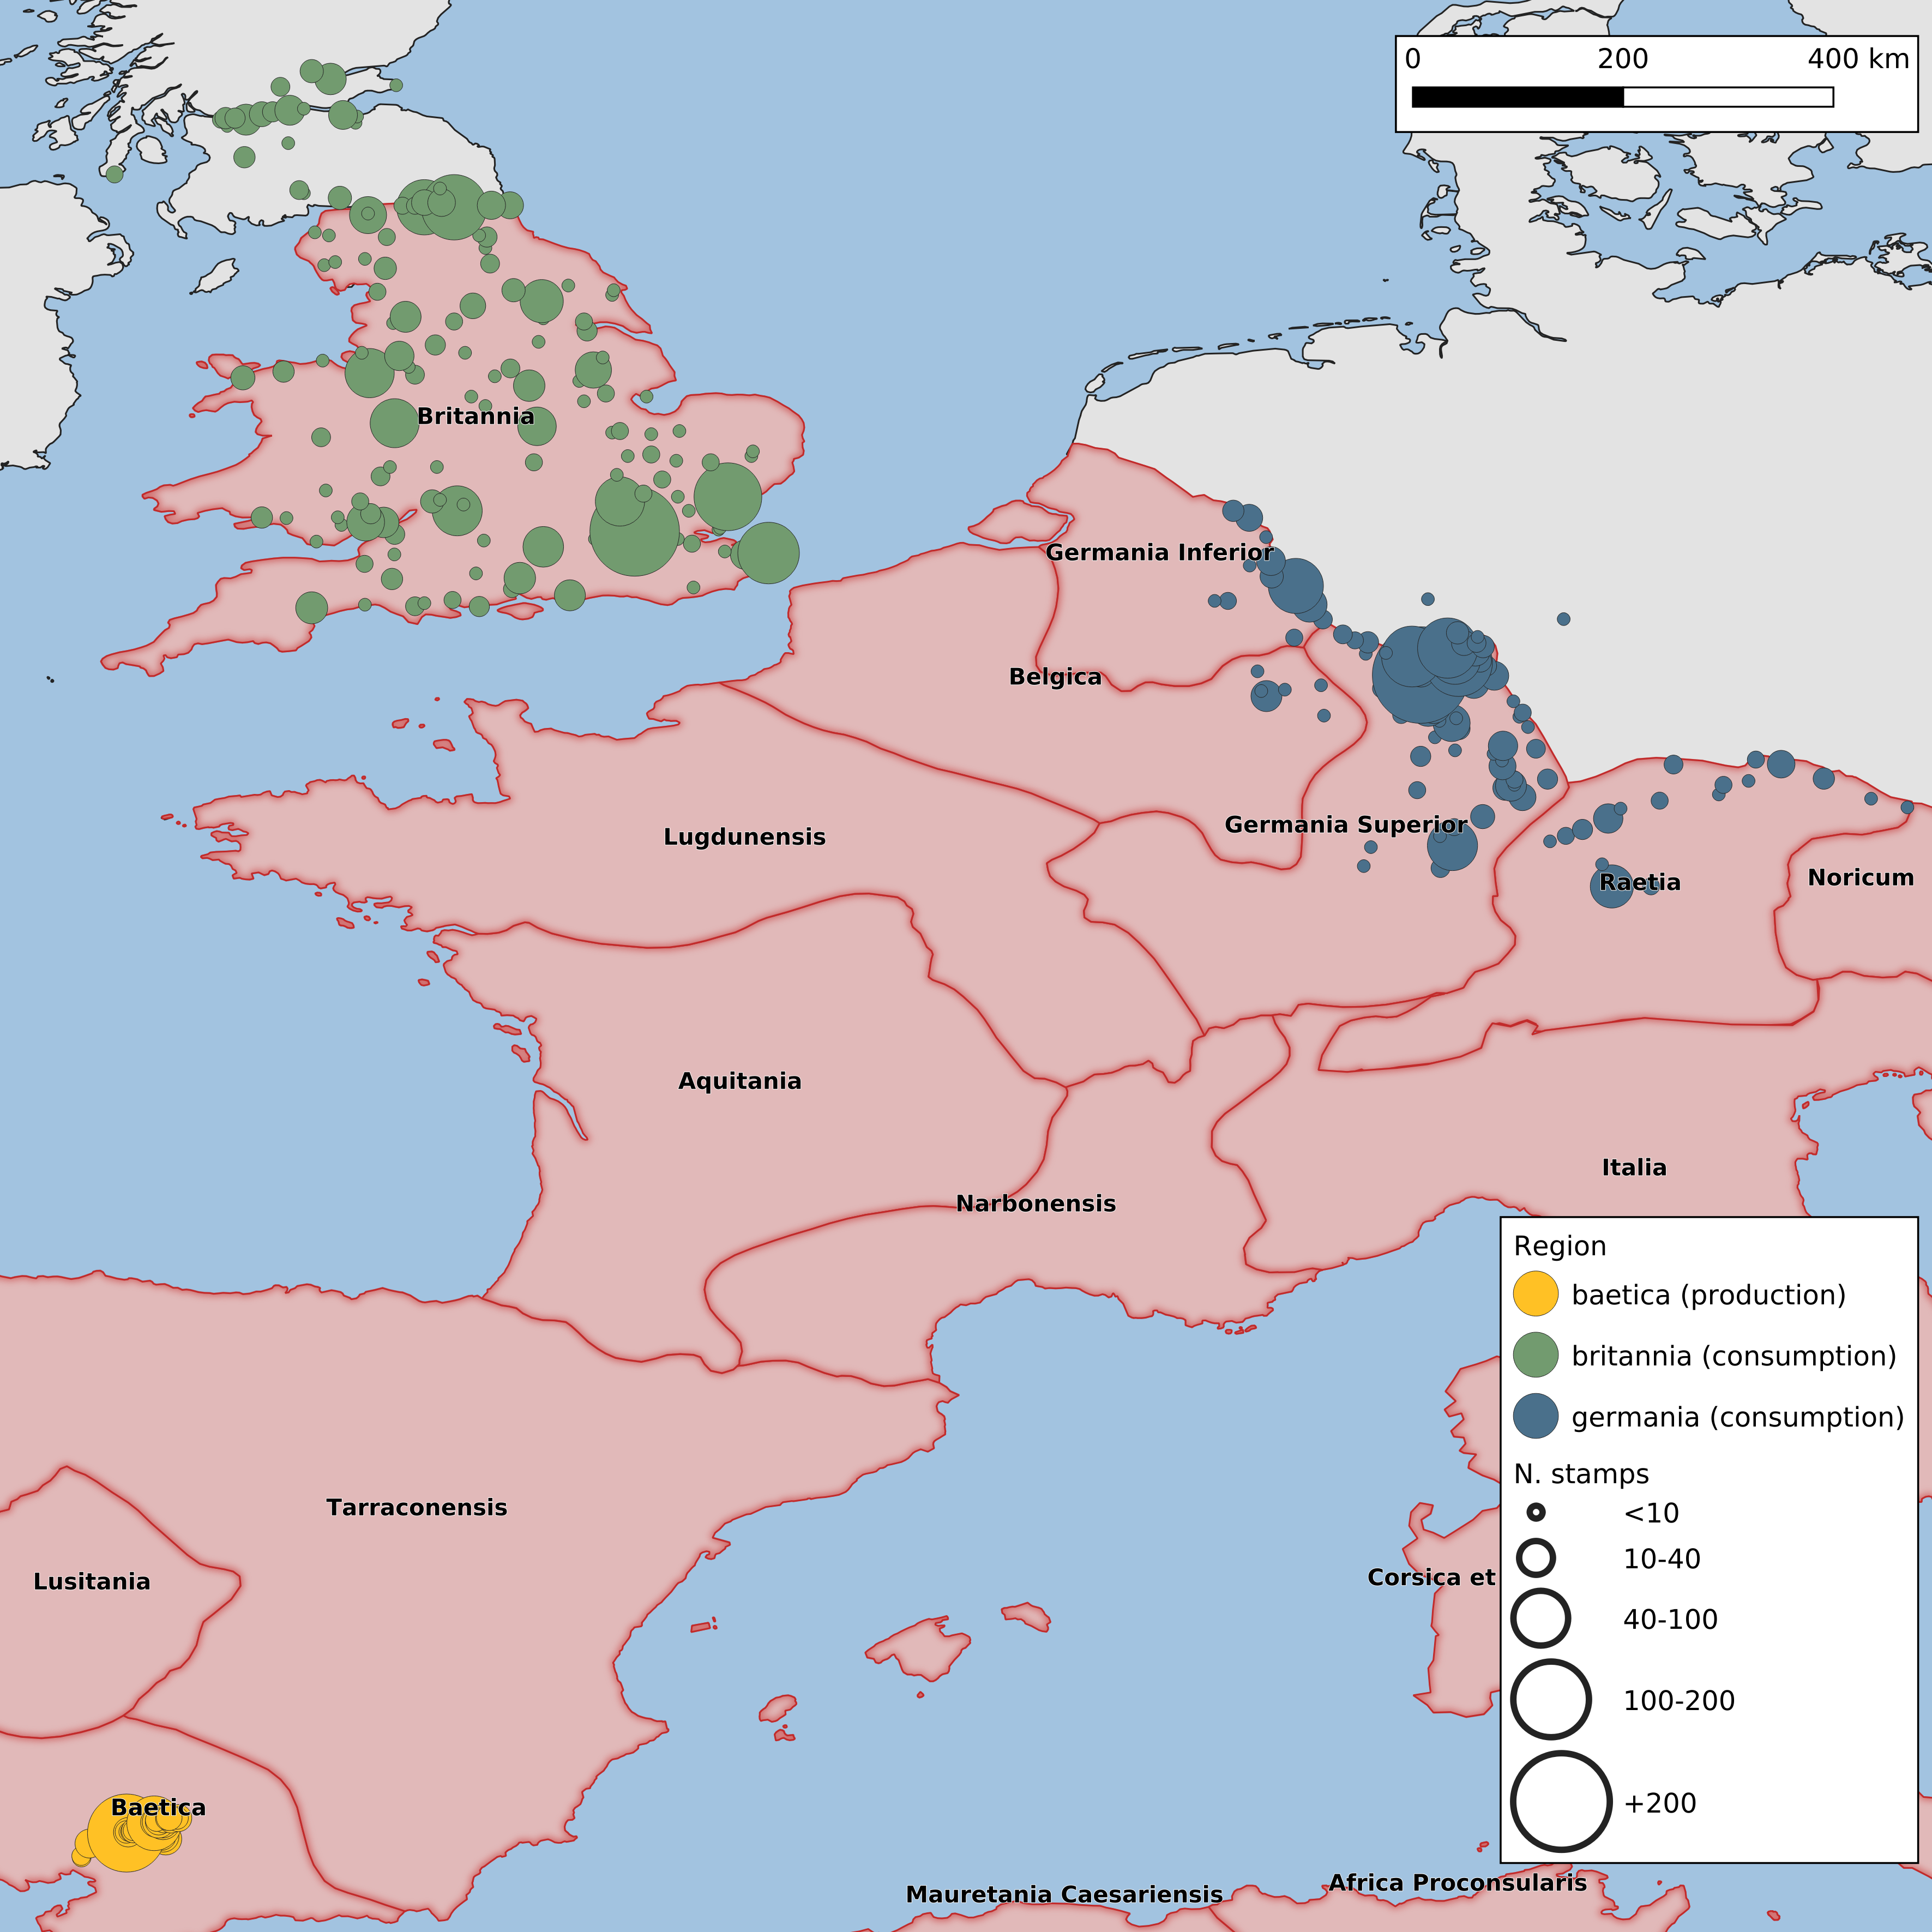
\includegraphics[width=\linewidth]{figs/general_map}
\caption{Overview of the sites analyzed in this paper. The color defines the three different regionsu under study (Baetica as producer; Germania and Britannia as consumers) while the size of each dot highlights the number of Dressel-20 amphoric stamps found on each of these sitese}

\label{general}
\end{figure} 
        
In the case of \textit{Baetica} province, we want to identify the role of the stamps in the organisation of the workshop; in Roman provinces, our aim is detecting groups of stamps concentrated in an area or if some groups have an important role for the exportation of olive oil in those provinces. This economic connection could be identified by different aspects: a) correlation between spatial distance and centres based on the idea that closer workshops concentrate similar amphoric stamps in a specific area than the distant workshops and b) groups of similar stamps were concentrated in a specific province. 

In particular, we study the distribution of amphoric stamps to identify a correlation between geographical distance and similarity. Based on this assumption, we proposed three hypotheses: a) we can identify a correlation between spatial distance and the distribution of stamps, b) stamps located in close workshops share similar traits and c) low mobility of amphoric stamps to other regions: stamps always stay in the same region.  

To do this, a population approach has been used to analyse the dispersion of stamps between amphora workshops \citep{rubio-campillo_ecology_2018}. Stamps will be used to identify economic patterns by analysing their similarity. If workshops and provinces share stamps with similar traits, then we can identify connections. By contrast, if we do not detect similar stamps between workshops, then workshops worked independently. 

The paper addresses these questions as follows: the next section introduces the historical context. Section two displays the dataset and the methods used for the analysis. Section three presents the results and the last section shows the discussion and the main conclusions of this work. 


\section{The Amphoric production of Baetica}

The landscape of the \textit{Baetican} province was one of the best regions to face the increase in demand of olive oil across the Roman provinces. For this reason the area saw an increase in productivity as a massive infrastructure of olive oil production was gradually deplyoyed. The production and distribution of olive oil grew exponentially\xavi{seguro que exponencial?} for almost three centuries\xavi{qué centuries?} \citep{remesal_concierto}. Hundreds of presses and amphora-making workshops were build near large extensions covered by olive trees. The workshops where amphorae were made and filled with olive oil were places along the rivers Guadalquivir and Genil riverbanks (see Fig.\ref{workshop}).

This strategic location allowed the transport of olive oil through riverine shipping towards the maritime routes that connected Baetica with Mediterranean and Atlantic trade routes towards the rest of the Empire\citep{garcia_vargas_enrique_formal_2010}.

\begin{figure}[htp]
	\centering
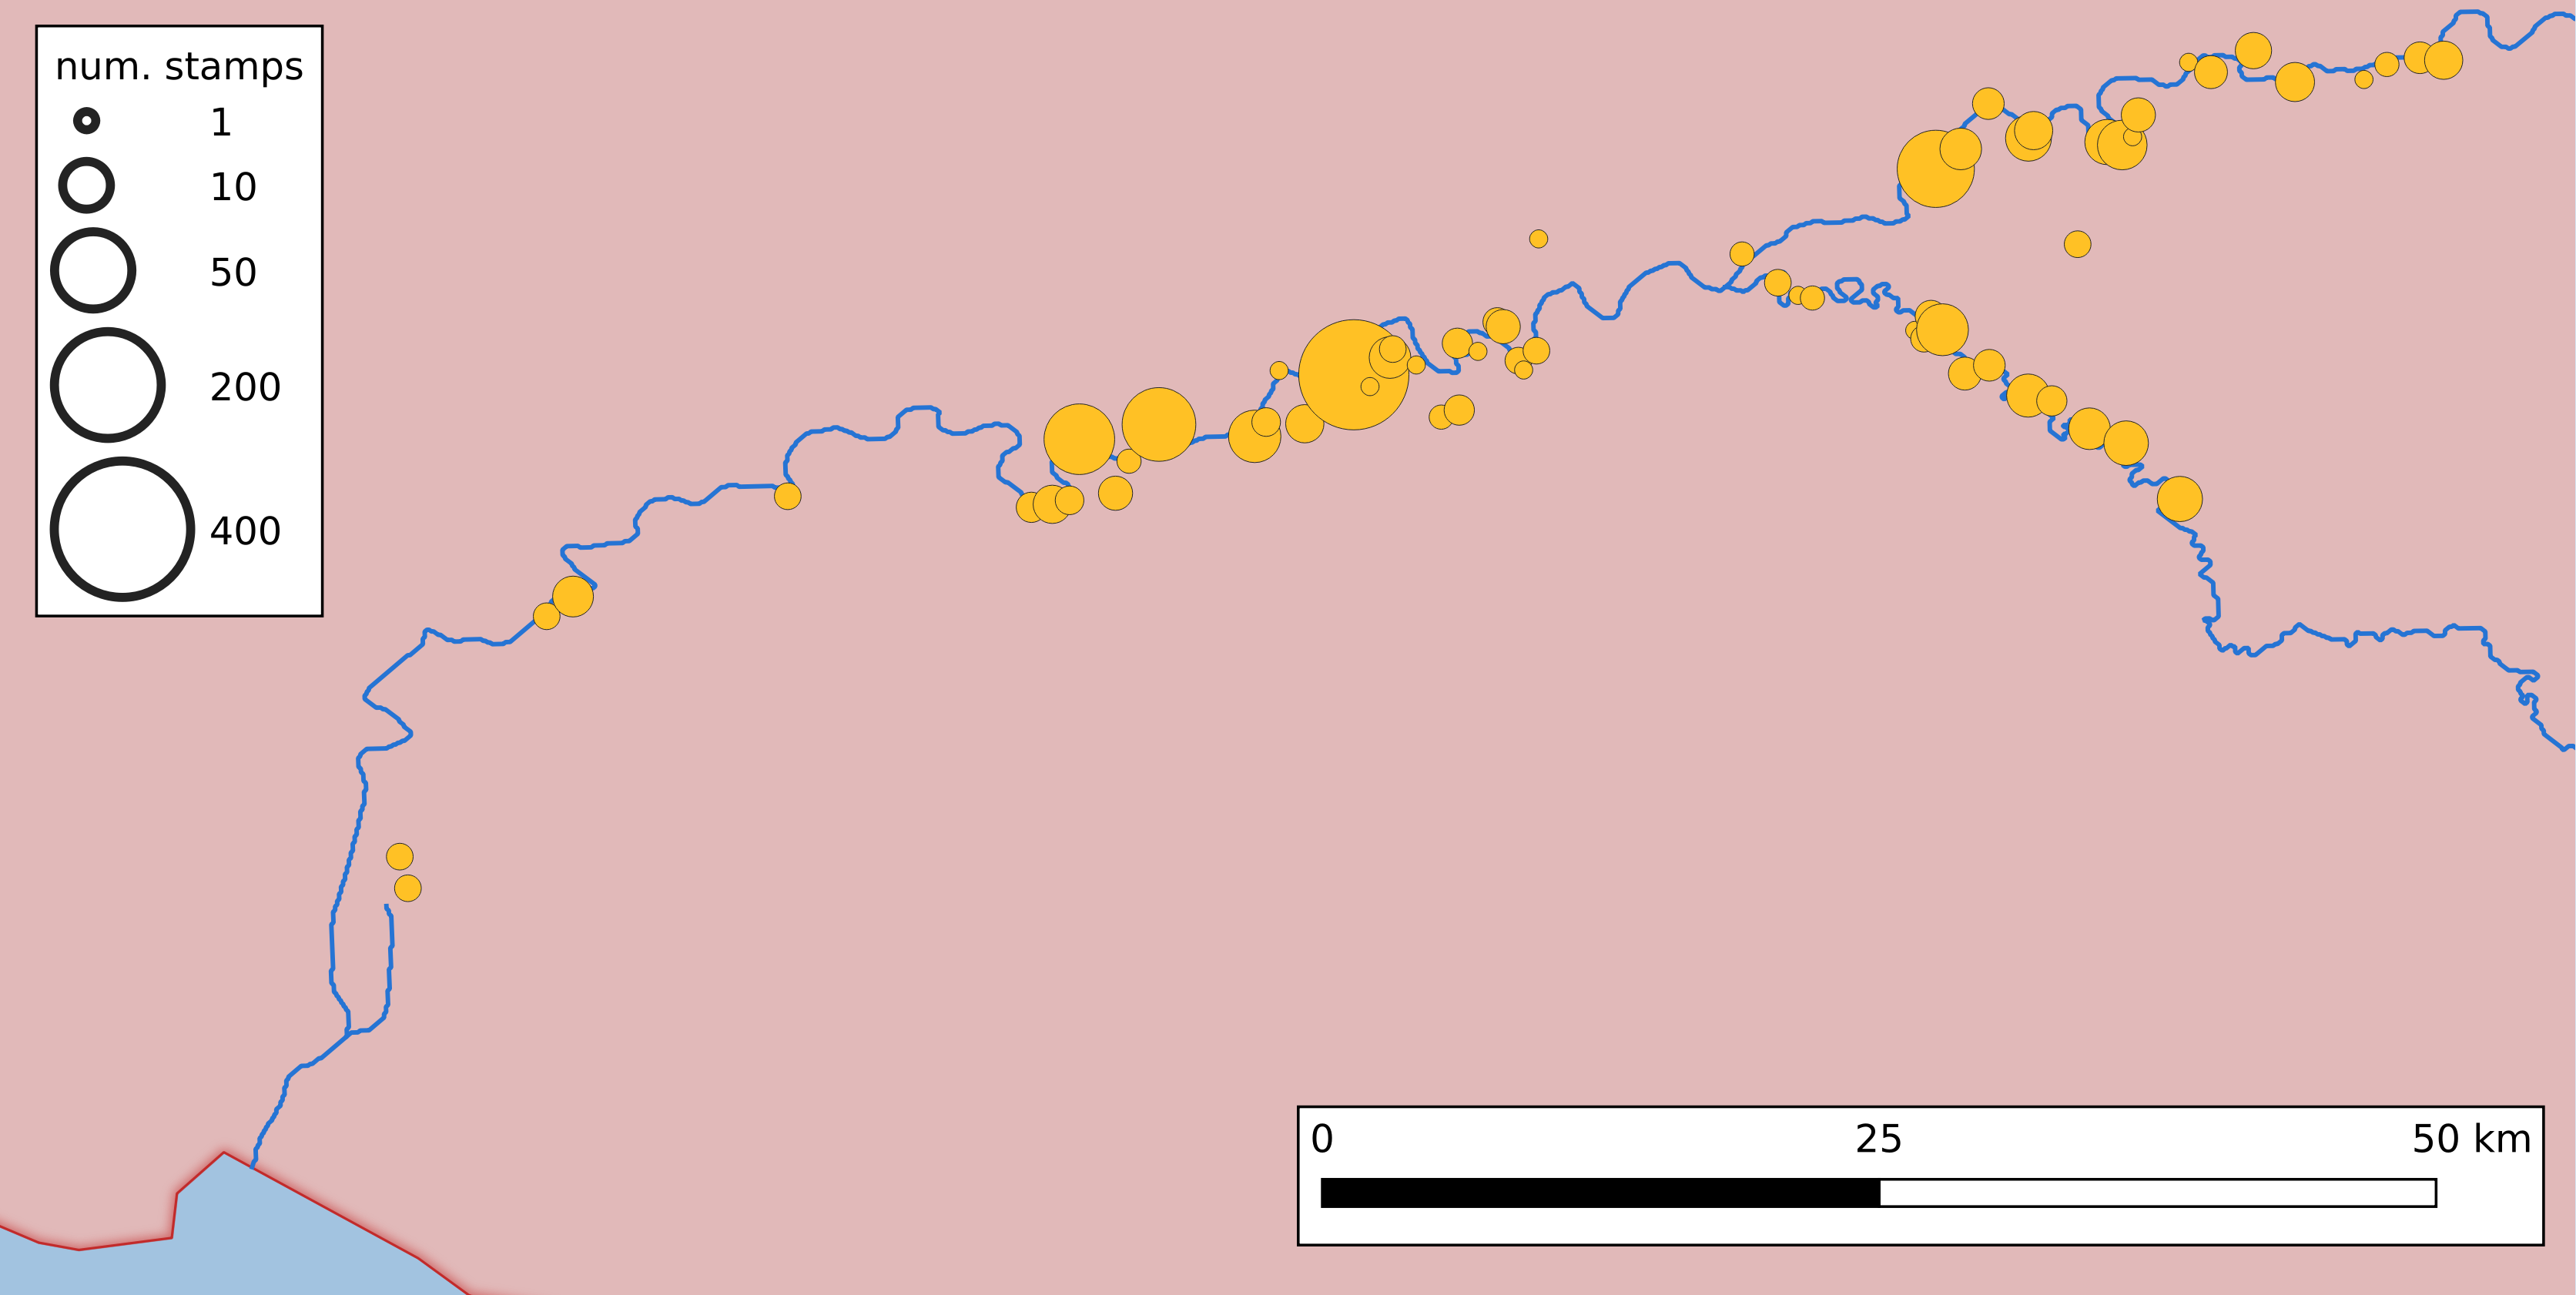
\includegraphics[width=\linewidth]{figs/baetica}
\caption{Distribution of stamps found in Dressel-20 workshops along the Guadalquivir riverbank. The size of each point depends on the number of stamps found on each site}

\label{workshop}
\end{figure} 


The chronology of the workshops is widely diverse from the first to the third centuries AD\xavi{qué quiere decir que la cronología es diversa?} \citep{millet_anforas_1998,rodriguez_baetican_1998,chic2005comercio}. 
This fact is shown by the archaeological evidence that displays a highly specialised production with a long activity with apparently few changes\xavi{deberías desarrollar esto un poco más; qué tipo de evidencia demuestra esto? pocos cambios en qué? los talleres? las tipologías anfóricas?} \citep{remesal_anforas_2004}.


A large majority of this Baetican amphorae production is composed by Dressel 20 types\citep{dressel_ricerche_1878,millet_anforas_1998}. Dressel 20 amphorae were shipped and distributed from \textit{Baetica} throughout western Europe\xavi{esto ya lo has mencionado; quizás podrías explicar en 2 líneas la capacidad y forma de la dressel 20}. 

Dressel 20 amphorae display a lot of evidence, but some of it is still hard to interpret. A large percentage of Dressel 20 were marked with stamps, while they could also be inked with \textit{tituli picti} or incised with \textit{graffiti}. The interpretation for most of these inscriptions is still open due to the fragmentation of the material and the small sample size of well-preserved elements~\citep{aguilera_evolucion_2007,rovira_guardiola_grafitos_2007}. 


%\xavi{Estás segura de esto? Porque aquí hay 2 cosas: 1. datar bien y 2 . período de uso. Yo no tengo claro que la mayoría de sellos se usen durante mucho tiempo. En qué está basada la idea? Deberías detallar un poco más este temita cronológico y explicar como sabemos el período de uso.}


%Some stamps show a more specific chronology while the majority of them display a large activity of production that it can be difficult for specifying an accurate chronology in some cases. This could be due to two reasons; firstly, most of the workshops were partially excavated and focused on archaeological surveys in order to collect the maximum stamps as possible; secondly, Dressel 20 was produced during almost three centuries with apparently few changes \citep{berni_piero_chapter_2017}.
 

\section{A potential indicator of Roman economy: Dressel 20 stamps}

Dressel 20 was the amphora most stamped during the Roman Empire \citep[18]{millet_anforas_1998}. The usage period is associated with a large amphora production for almost three centuries\xavi{esto está repetido no?}. 

The large sample size of recovered Dressel 20 stamps is distributed across all the western provinces of the Roman Empire. For this reason there are several publications of this type of evidence discussing its origin, its meaning, its long period of use and its spatial distribution~\citep{remesal_sellar_2016} (Fig.\ref{amphora}).\xavi{si dices que es muy popular debería haber aquí más citas aparte de Remesal}. 

\begin{figure}[htp]
	\centering
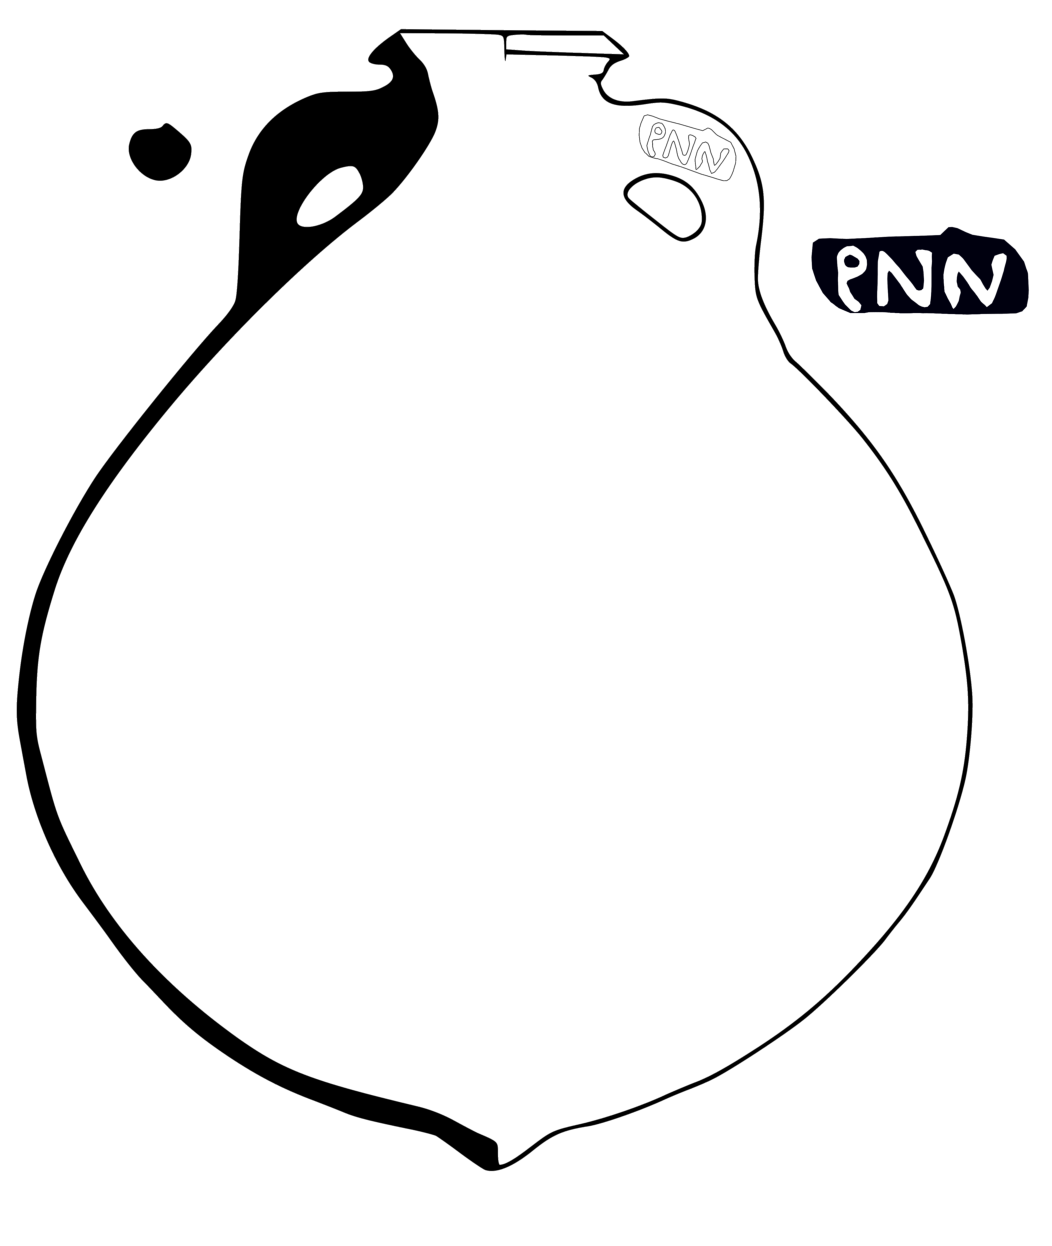
\includegraphics[scale=0.5]{figs/dressel20}
\caption{Dressel 20 were mostly marked with stamps of three letters called \textit{tria nomina}}
\label{amphora}
\end{figure} 

Most stamp codes display a large activity of production that can be difficult to date using an accurate chronology. They have been frequently dated with the consular dating by studying \textit{tituli picti} found in \textit{Monte Testaccio} \citep{Testaccio1, berni_millet_epigrafianforica_2008}. However, the chronology of stamps could be also biased in other sites taking into account that amphorae were deposited after being produced and consumed\xavi{esto necesita un poco de desarrollo. quieres decir que el código se encuentra en contextos de cronologías diferentes no? Y lo del Testaccio, pos eso, que hay pocos y todos de un yacimioento, lo que añade un bias}.  

These stamps are typically found on handles but they were also imprinted on rims and the amphora body~\citep{millet_anforas_1998}. The information of the stamps is shown in different forms and letter content and it seems that there was not a unique criterion\xavi{qué information? El código de letras?}. Stamps often displayed a code of three letters and they can appear in abbreviated form or complete and they are known as \textit{Tria Nomina} \citep{berni_millet_amphora_1996}.\xavi{que quieres decir con abbreviated o complete? Como abrevias un código de 3 letras?}

Scholars agree that stamps are some type of identification mark, but there is no consensus on the meaning of these marks\citep{rodriguez_baetican_1998}. Additionally, a large percentage of Dressel 20 containers were not stamped thus complicating the interpretation~\xavi{esta última frase aquí es un poco random no?}. The stamp codes are interpreted based on three main ideas: content (olive oil), context (amphora workshop) and subject (individuals involved on the production). On the one hand, it seems that stamps could have been identified as the landowner of the olive groves \citep{rodriguez_economioleicola_1977}. On the other hand, they could also belong to the owner of the workshops were the amphorae was made or even to a group of amphora workers~\citep{berni_millet_epigrafianforica_2008}. In any case, the use of these stamps is a good proxy to explore the system of olive oil production and trade developed in Baetica.

Nevertheless, some challenges\xavi{acabas de decir que tampoco se sabe qué es el sello, así que esta frase queda rara} remain under discussion such as how this production was organised and whether it is possible to distinguish production patterns in the olive oil trade. Our questions will be focused on the distribution of amphoric stamps. Did they follow a distribution pattern? Did stamps share the same workshop? 

Neither the use of written records have allowed providing enough information that can explain the economic role of \textit{Baetica} province in the Roman organisation.\xavi{esta frase esta fuera de contexto. Si la pones entonces deberías expandir la idea de frase a párrafo, y poner referencias}.
  


%\subsubsection{Jaccard distance}
%The dataset was analysed using a statistic method as Jaccard distance. This method allows to measure the dissimilarity by calculating the presence of sets (CITAR). In our case, Jaccard distance was used to compute the mutual presence of traits in the amphora stamps but it does not consider the number of absences. A comparison was done with the distance of the workshops to identify whether there was an association between stamps and spatial distance amongst workshops. 

\section{Case study: consumption centres}

\xavi{este título es muy raro, porque 1. que son casos de estudio ya lo sabes y 2. case study singular, consumption centres plural}

The creation of new provinces allowed the Roman Empire the arrival of resources through Mediterranean and Atlantic routes\xavi{no entiendo esto...allowed o required?}. This led to a gradual change in the economic and social structureas the trade networks that supplied the Roman army became more complex. Augustus's administration created the figure of the \textit{praefectura annonae} to organize wheat supply. The role of the \textit{praefectura annonae} was mainly focused on providing through \textit{frumentationes} a fixed monthly amount of wheat to each Roman citizen~\citep{remesal_annona_1986,remesal_concierto}\xavi{pero estabas hablando del ejército no? Has hecho un salto aquí a los ciudadanos}. 

Some authors argue elsewhere that this same \textit{Annona} could also have organized the supply of additional goods such as olive oil to the Roman legions \citep{remesal_annona_1986,remesal_annona_1990}\xavi{pero no hay evidencia? Las fuentes escritas no lo mencionan?}.

The importance of this olive oil trade is revealed by the massive amount of Dressel 20 amphorae found across the Roman provinces. This amphora has been commonly associated with the transportation of Baetican olive oil for supplying military camps and civil settlements \citep{berni_millet_epigrafianforica_2008}.\xavi{me parece repetitivo, porque unos párrafos antes ya hablabas de lo mismo. Quizás unificar texto aquí o allá?}
 
The military consumption of olive oil in Roman provinces may be related to two aspects: a) cultural consumption whose product is consumed by cultural reasons such as to identity or habit and b) economical reasons where olive oil distribution is based on the transport costs, unlike other products \citep[69-70]{carreras_britannia_1998}\xavi{no pillo esta frase}.. 

Olive oil supply seems to be particularly intense in militarised provinces that functioned as the borders of the Empire such as \textit{Britannia} and \textit{Germania}. The high percentage of amphorae\xavi{amphorae o Dressel 20?} found in sites nearby military garrisons suggests the existence of diverse supply dynamics as there were trade processes flowing good from military sites to civil settlements\citep{remesal_annona_1986, carreras_britannia_1998}\xavi{lo que quieres decir es que tienes muchas ánforas en sitios civiles cerca de militares? no queda claro}.

\xavi{faltaría un enlace a la siguiente sección, queda muy abrupto}

 
%\xavi{este título de sección debería cambiarse por algo más descriptivo. Case studies o algo asínnn? Por otra parte, igual podrías dividirlo en 2 subsections}

%\xavi{en general, echo a faltar un poco más de detalle en esta discusión y en los datos que tienes; en qué se parecen y diferencian las 2 provincias? Si hablas del uso por las campañas o las guarniciones, donde están? Qué strategic points de redistribución hay? Tampoco a saco, pero entender mejor cómo llega el aceite, cómo se redistribuye y quién y dónde se consume}

\subsection{Britannia}

The evidence for olive oil consumption in \textit{Britannia} is scarce before the Roman conquest \citep{funari_corpus_1996,carreras_abastecimiento_2003}. Indigenous\xavi{no sé si indigenous es la mejor palabra...local?} population did not consume this product and it was not produced on the region as the landscape and climate of the British isles was not suitable for olive oil trees\citep[161]{monfort_britanniaen_1998}. Based on the archaeological record this absence of olive oil changed with the arrival of a large amount of Dressel 20 amphorae to \textit{Britannia} \citep[1]{carreras_britannia_1998}\xavi{en qué siglo?}. The demand of olive oil after the Roman conquest required of a new trade route due to the lack of local olive oil production; \textit{Baetica} was chosen as its main supply.

At this moment, we detect an increase of the olive oil exportation concurring with the displacement of legions during the military campaigns \citep[161]{monfort_britanniaen_1998}\xavi{repetitivo? fusionar párrafos}. This fact will have a particular intensity within sites close to the Hadrian Wall's garrisons.  Olive oil production in \textit{Baetica} would cross the Atlantic until they reached the province and redistribute throughout the area from a series of strategic locations~\citep{carreras_atlantic_2012}. The increase of the exportation of Dressel 20 amphorae created an important commercial network for exchanges. Thus, the network was mainly focused on the support of soldiers during military campaigns\xavi{estas 2 frases repiten cosas ya explicadas}. 


The presence of Dressel 20 stamps in military camps in \textit{Britannia} has been widely studied in Roman archaeology \citep{carreras_britannia_1998}.\xavi{si dices widely studied no puedes referencias solo 1 autor}. This fact\xavi{que fact? Que los sellos de dressel 20 han sido muy estudiados? No tengas miedo a repetir trozos rollo "This intense consumption of olive oil also indicatas blablabla...} also indicates a possible provincial structure designed to organize the supply of olive oil to military camps,m such as \textit{Germania} (Remesal Rodrıguez, 1986)\xavi{por qué such as Germania? Aún no has explicado qué hacen en Germania}. There are no written records explaining how this redistribution of essential goods was organised in \textit{Britannia}, but the archaeological evidence suggests that cities may have been the central nodes of this local trade network~\citep[45]{funari_economic_2005}.

The consumption of olive oil would experience a progressive slowdown from the third century A.D. onwards. This date matches a change in market strategy in the Empire. This a gradual decrease on \textit{Baetican} olive oil exports can be observed as a decrease in the amount of Dressel 20 found in excavated sites as this typology is replaced by Dressel 23 amphorae \citep{rodriguez1991aceite,millet_anforas_1998}.\xavi{pero entonces la dressel 23 de donde viene? Cuidao que estás diciendo que se acaban las dressel 20, pero esto implica que hay menos aceite de oliva o que viene de otras partes o que va en recipientes distintos a la dressel 20?}

\subsection{Germania}

Julius Caesar's campaigns in \textit{Gallia} during 1st BC opened the door to the invasion of \textit{Germania} during Augustus rule~\citep{remesal_annona_1986,remesal_baetica_2002}\xavi{no hay un resumen de la conquista similar para Britannia, queda raro}. Previous studies suggested that the supply to the German limes was mainly based on riverine transport, but recent works suggest that the maritime route through the Atlantic Ocean could have been more important than expected (both for Germania and Britannia).~\citep{remesal_germn_2010,rubio-campillo_ecology_2018}.\xavi{lo del océano atlántico está un poco descontextualizado; no sería mejor ponerlo al final de esta sección?}

Roman studies exploring the presence of Dressel 20 amphorae in \textit{Germania} has not had the same impact as the rest of the province\xavi{no entiendo esta frase. Que qué provincia? Germania son 2 provincias no?}. This could be explained due to the lack of archaeological sources \citep{horacio2010llegada}. As a consequence, it is still unknown if trade agents participated on the distribution of Baetican olive oil in \textit{Germania} or the supply was exclusively focused on the Roman army garrisons\citep[156]{remesal_germn_2010}\xavi{quieres decir que aquí sólo encontramos dressel 20 en yacimientos militares porque no se han excavado muchos civiles?}. 

\textit{Germania} presents a similar introduction pattern of olive oil than the one discussed for \textit{Britannia}. There is no archaeological evidence for olive oil consumption before the arrival of the Roman army to the region while a majority of recovered Dressel 20 amphorae are located in the military sites that formed the German \textit{limes}\xavi{cita?}. 

The presence of the Roman army encouraged the exchange in the province as shown by the arrival of this product both civil settlement and military sites with a mayor concentration at the German \textit{limes}\xavi{pero justo antes decías que no había en civiles no?}. It seems that some Baetican centres would be assigned to the support of olive oil\xavi{the support of olive oil no se entiende. Además, falta alguna cita y desarrollar esta idea}. However, this hypothesis is hard to assess given the current lack of archaeological evidence \xavi{related to BLABLABLA. Habría que detallar un poco porque hay un montón de evidencia arqueológica del limes, así que qué es exactamente lo que falta?}\citep[125]{remesal_concierto}. 



\section{Material and Methods}


The goal of this study is exploring the effect of the production patterns between different centres. We are especially interested in identifying links between production and consumption centres by using amphoric stamps. To do that, we use the CEIPAC database to collect stamps from different places. The CEIPAC dataset contains over 50.000 of epigraphy records found in amphorae, mostly from \textit{Monte Testaccio}.
This study proposes a robust baseline to explore the distribution of Baetican olive oil production by computing the spatial correlation between stamps. A way to analyse is to use a quantitative framework to measure the similarity between amphoric stamps. Here we use an ecological approach based on three steps: a) to detect similarities between stamp codes, b) to explore a potential spatial correlation and c) to establish a correlation between similarity of stamps and spatial distance. 
\xavi{estos 2 párrafos explican objetivos, que deberían ir en la intro y no aquí, donde deberías empezar a hablar directamente de la BBDD}


\subsection{Production centres: Baetica province}

To study the stamps found in the Baetican workshops we used the data collected in the CEIPAC database of amphoric epigraphy~\citep{remesal_centro_2015} (see the database here \url{http://romanopendata.eu}). This database contains over 50.000 epigraphy records found on different types of amphorae\xavi{podrías mover esta parte a los 2 párrafos anteriores y explicar la bbdd brevemente antes de empezar a hablar de la Bética (porque es info que también aplica a los otros 2 casos de estudio no?}.

There databased allowed us to retrieve 3798 stamps found in Dressel 20 amphorae recovered from workshops within \textit{Baetica} province. Each of these stamps ha detailed records on the site where it was found, the inscribed code as well as its spatial coordinates. The stamps with incomplete information were discarded, thus finishing with a sample of 987 stamps from 81 sites and displaying 130 different code.

%Approximately 70 \% of stamps cannot be tested due to the fragmentation of the dataset. Consequently, any stamps with incomplete information were discarded and not integrated into our dataset. 

Our dataset also contained a new categorical variable defining the \textit{conventus} of each site. The \textit{conventus} were administrative centres for territorial organisation in the Roman Empire \citep[58]{ozcariz_gil_administracion_2013}\xavi{estaría bien ampliar un poco esto; qué organizaban exactamente?}. The production area for Dressel 20 amphorae extended across three different \textit{conventus}: \textit{Hispalensis} (currently Seville, hereafter Hispalis), \textit{Cordubensis} (currently C\'ordoba, hereafter Corduba) and \textit{Astigi} (currently Écija, Sevilla, hereafter Astigi) \citep{rodriguez_economioleicola_1977,chicdatos2001,berni_millet_epigrafianforica_2008} . 

%3798 = base de datos sin limpiar
%3791 = base de datos limpiada con cleanstamp.py
%3787 = no sé a qué corresponde pero es archivo baetica.csv

It is important to mention that some workshops exhibited the same coordinates but they were catalogued as different workshops in Roman Studies (i.e. Tesorillo de Doña Mencia and Doña Mencia). The analysis took into account this particularity but some biases can occur due to the archaeological dataset\xavi{No se entiende; deberías explicarlo un poco mejor y citar algo si dices eso. Piensa que la mayoría de lectores no sabrán quién es Doña Mencia}. 

The first step was to compute the frequency distribution of stamp codes and analyse it using Exploratory Data Analysis (EDA). This would allow us to study the distribution of the stamps across centres as can be seen in Figure~\ref{stamps}. Most workshops contained only one stamp~\xavi{el gráfico es dificil de entender...yo leo que hay unos 20 workshops con 1 solo stamp, por lo que entiendo que no es cierto que la mayoría solo tengan 1 sello (hay como 50 workshops con entre 2 y 30 sellos no?)} One workshop (La Catria) concentrated a large percentage of the amphoric stamps with a total number of 228 stamps. The type of distribution is also frequent in amphora production where we observed a self-organised complex system pattern with a major concentration of the number of stamps in a few workshops \citep{bayesian_2018,coto-sarmiento_identifying_2018}\xavi{no lo veo; recuerda que para el rollo bayesiano tenías una línea recta al hacedr el log de los 2 ejes, no solo 1, y este plot no está construído así no?}.

%The type of distribution is also frequent in the Roman economy where we observed a self-organised complex system pattern typical of a free market 

%\xavi{que me quede claro...la mayoría de workshops solo tienen 1 sello??? Y hay un workshop con como 700 sellos distintos??? }

\begin{figure}[htp]
	\centering
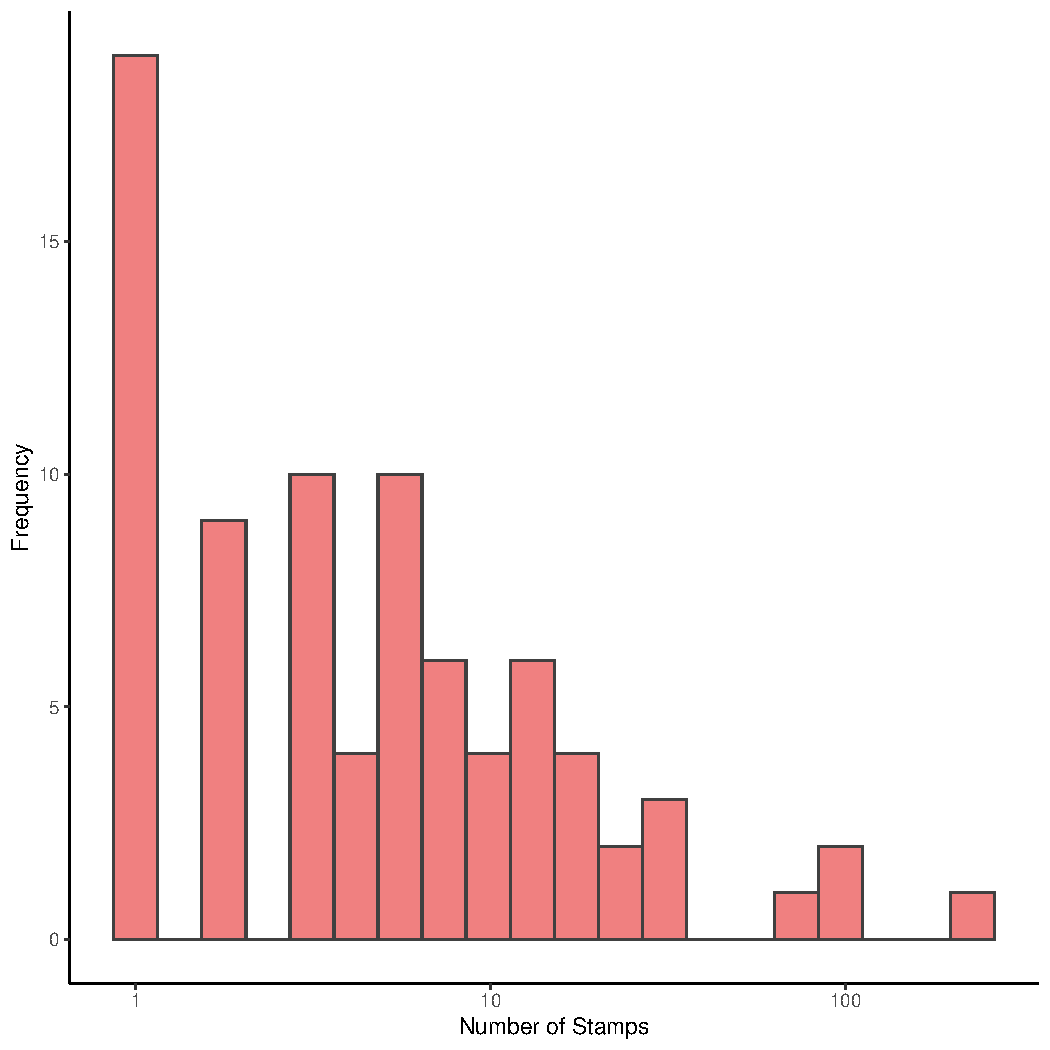
\includegraphics[width=\linewidth]{figs/frequencystamp.pdf}
\caption{Histogram on a log scale with base 10. X axis is represented by the number of stamps and Y axis is the frequency of workshop. The distribution is widely diverse with most workshops having only one stamp}
\label{stamps}
\end{figure} 

%\xavi{si el eje es logarítmico deberías mencionarlo}


The distribution of amphora stamps for each \textit{conventus} can be seen in Figure~\ref{frequency}. The majority of stamps are concentrated in \textit{Hispalis} (574 stamps) while \textit{Corduba} and \textit{Astigi} have roughly half this sample size (267 and 146 stamps). The workshops of the three conventus show a similar pattern on the stamp frequency distribution with the exceptions of 2 large workshops in \textit{Hispalis} (La Catria and Arva). On these two workshops a comparatively large amount of stamps were found (29 different code stamps on each of them)\xavi{una cosa, aquí has pasado de sellos a códigos, y los valores son distintos que en el gráfico anterior. Deberías clarificarlo antes de empezar a hablar de la figura}. According to previous studies those workshops became the most important centres of amphora production in the region\xavi{cita de estos estudios}. It is worth mentioning that a majority of these stamps were collected during ield surveys with no excavation, so this difference in sample size could be biased due to differences in intensity across the different sites~\citep{arva_1997}.
 
\begin{figure}[htp]
	\centering
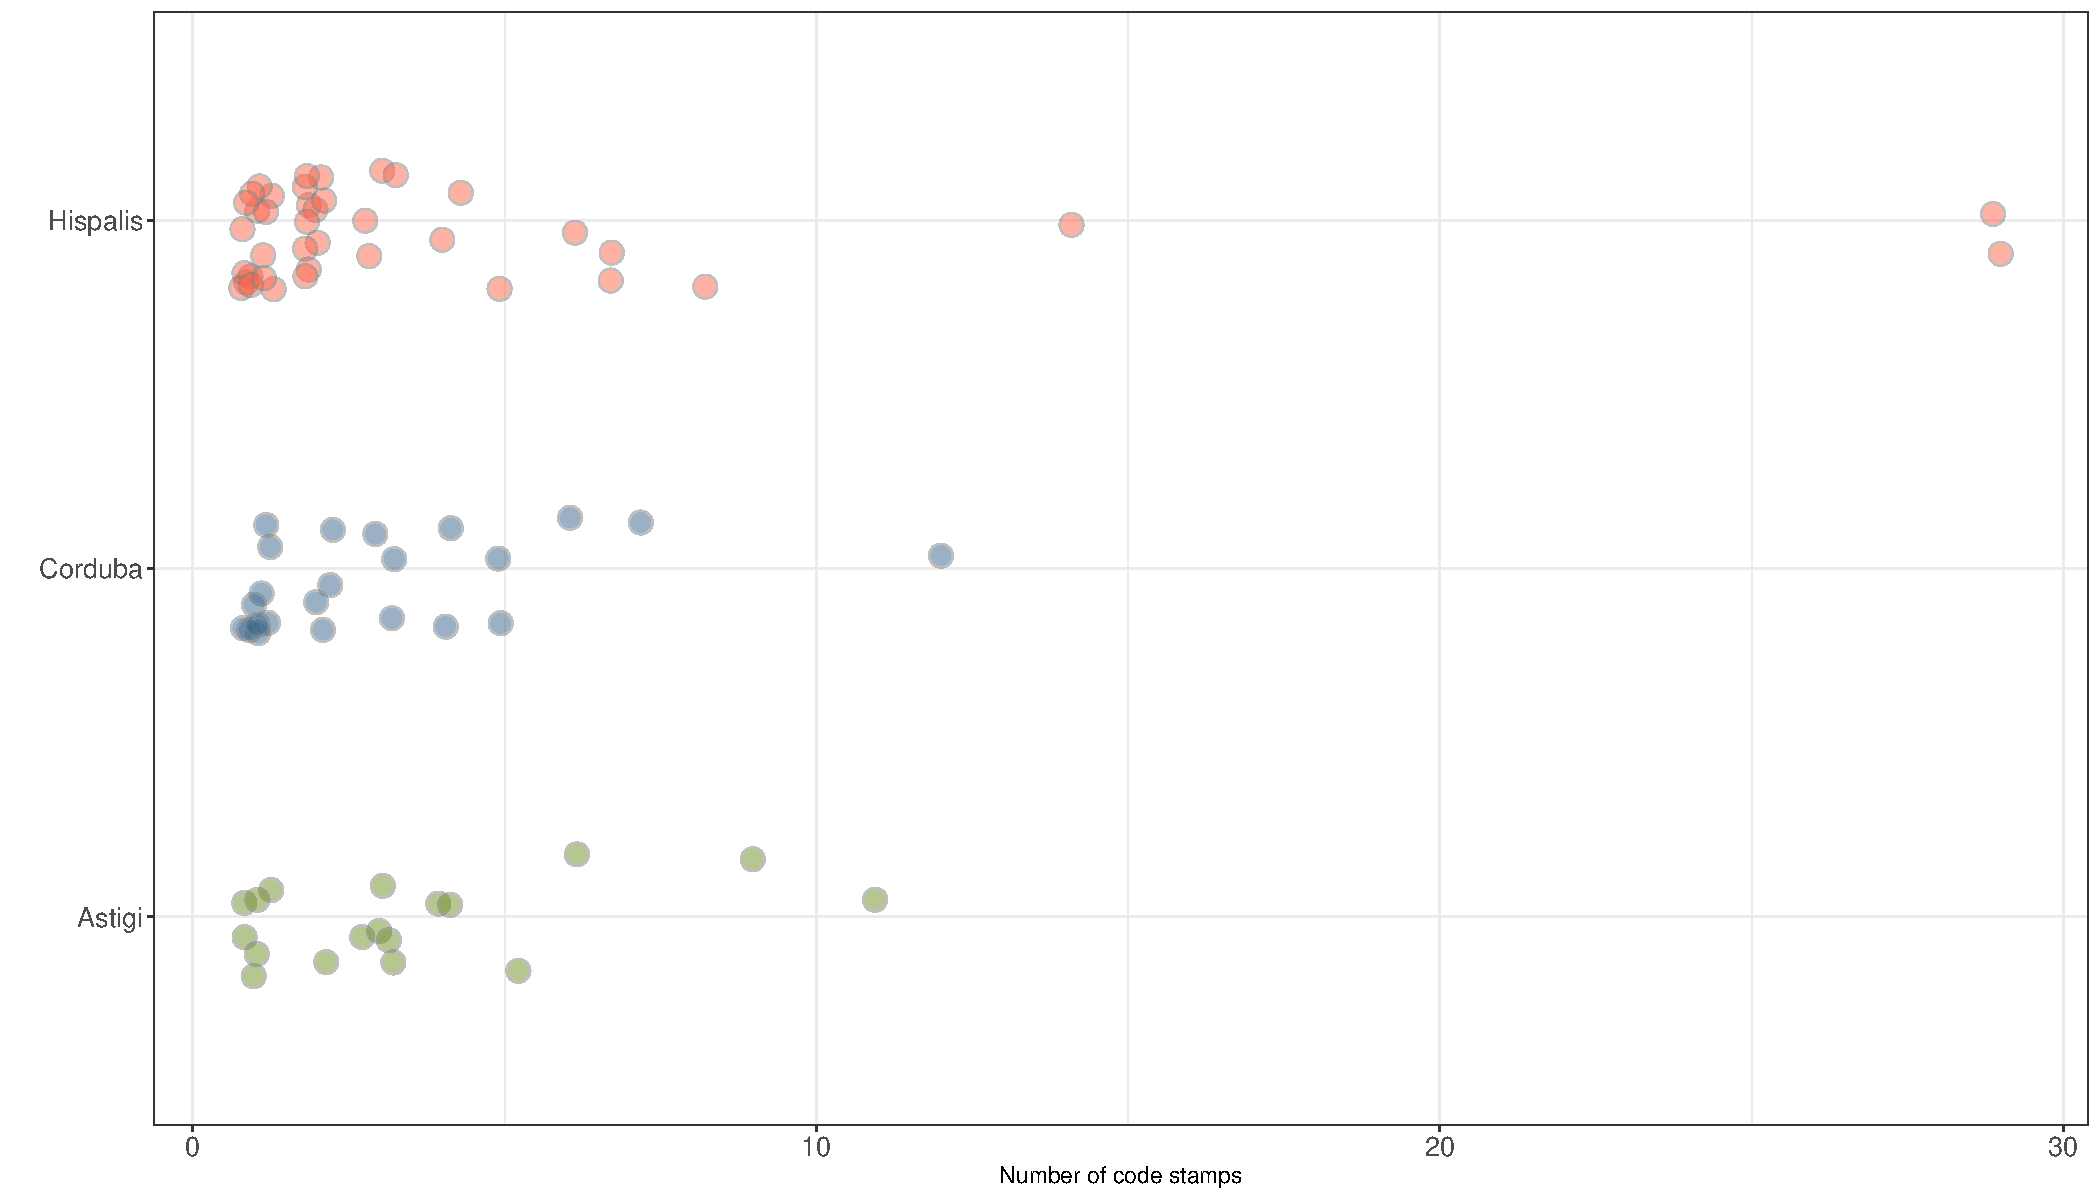
\includegraphics[width=\linewidth]{figs/frequency}
\caption{Distribution of the number of different code stamps (X axis) for each \textit{conventus} (Y axis). Each dot corresponds to a workshop sorted by different areas. Colours are represented by areas divided into Hispalis (red), Astigi (green) and Corduba (blue)}
\label{frequency}
\end{figure} 

%\xavi{vale pero qué es cada punto? un workshop?}


\subsection{Consumption centres: Britannia and Germania}

%\xavi{Esta estructura no me convence...tenemos que pensar algo mejor, porque ahora es: 1. hablo de britania/germania, 2. hablo de sellos en general, 3. hablo de sellos en britania/germania. Quizás juntar esto con lo de los casos de estudio, o quizás hablar de los 2 casos de estudio en la intro, y dividir la sección anterior en 2 (lo más general a la intro, lo más concreto aquí)}
The analysis of stamps in consumption areas also used the CEIPAC database and filtered in the same way than the previous dataset. We selected the centres with more or equal than five stamps\xavi{pero esto no se hizo en el de Baetica no? Por qué?}.

The output was a dataset of 4271 stamps found in sites belonging to \textit{Britannia} (2219 stamps) and \textit{Germania} (2052 stamps). Both \textit{Germania} and \textit{Britannia} were analysed as borders and not as Roman provinces. This means that we included in the sample some centres that are actually located beyond the administrative boundaries but were considered part of the same border. Specifically, for the German \textit{liomes} we included sites from the two provinces (Ulterior and Citerior\xavi{no es superior e inferior?}) while the analysis of Britannia extended to \textit{Caledonia}.
 
%We analysed a dataset of 2219 stamps from different centres in \textit{Britannia}. 
%CITAR (Callender, 1965; Carreras Monfort y Funari,1998; Ayllón-Martı́ et al., 2018). 
In \textit{Britannia}, we studied a total sample of 1765 stamps from 46 sites displaying 968 unique codes\xavi{pero esto no concuerda con las 2219 de antes...es por descartar los inciertos? Hay que dejarlo claro}. The centres located in \textit{Britannia} can be seen in Figure~\ref{britannia}.
 
\begin{figure}[htp]
	\centering
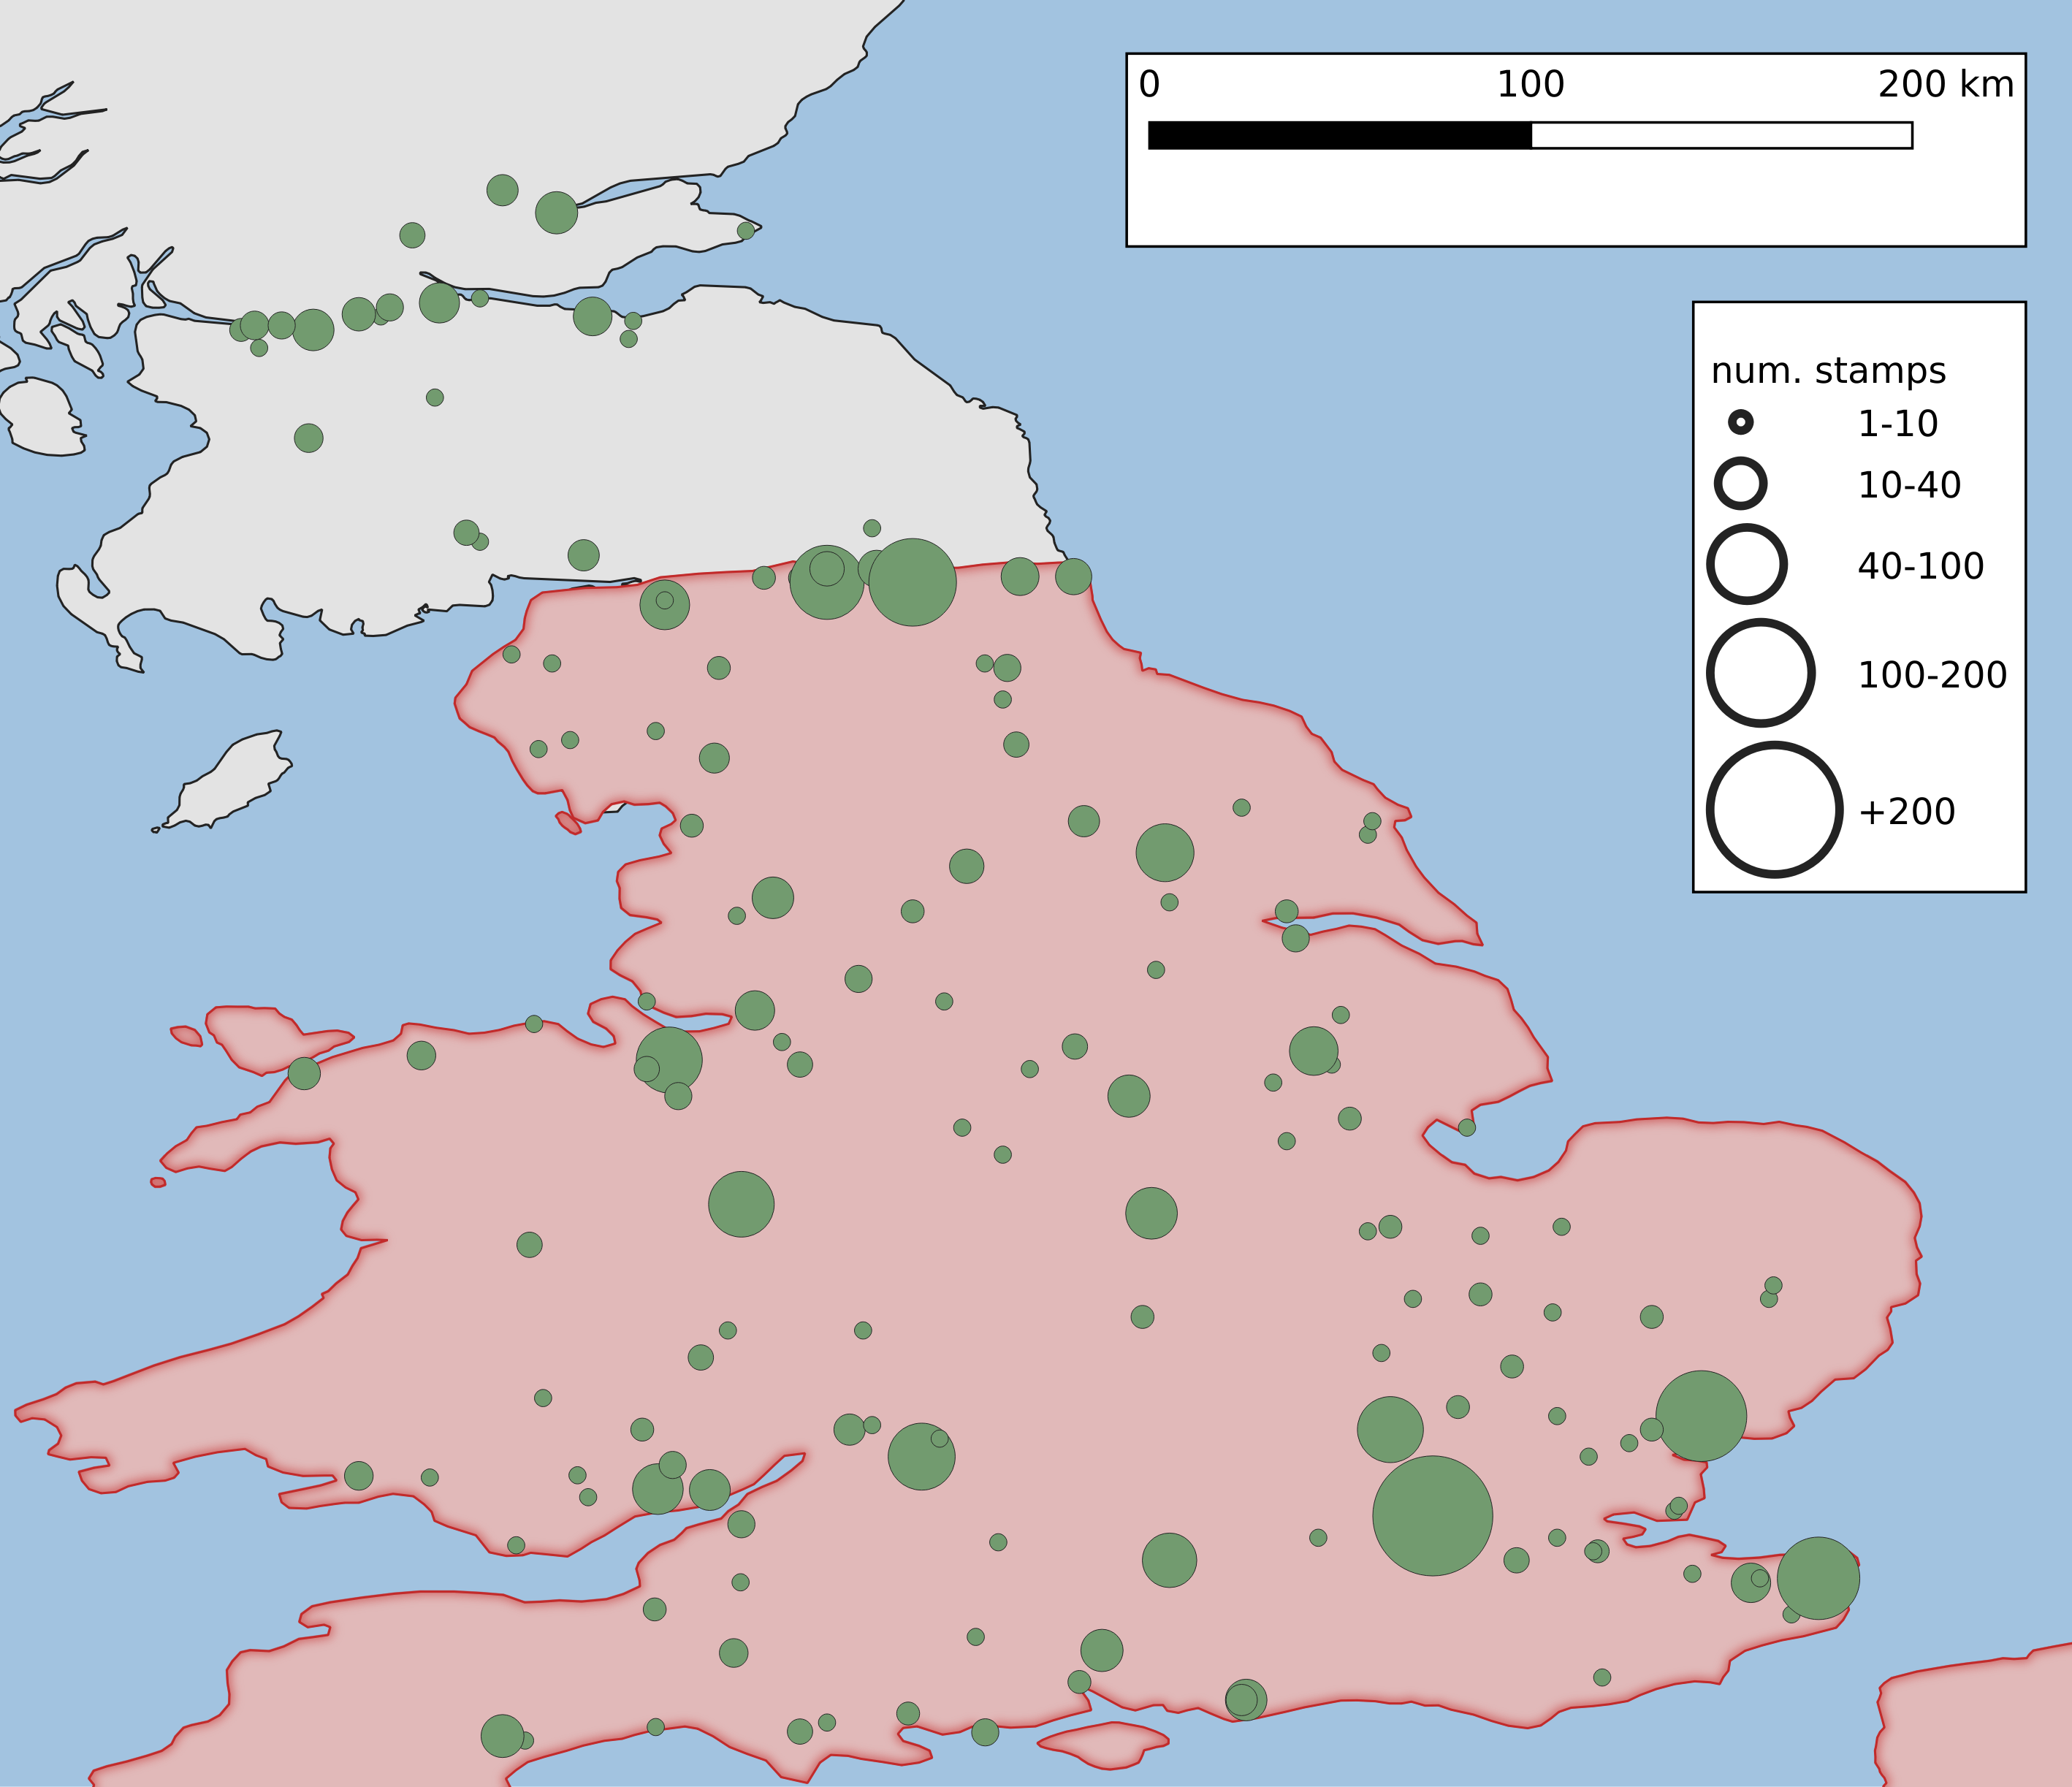
\includegraphics[width=\linewidth]{figs/britannia}
\caption{Sites in Britannia where Dressel-20 amphoric stamps have been found. Each dot is a site while its size shows the sample size of stamps found in the site. A majority of stamps have been found in garrisons related to Hadrian's and Antonine walls}
\label{britannia}
\end{figure} 


%We analysed a dataset of 2052 stamps placed in \textit{Germania}. All the data was also compiled by CEIPAC database. As previously before, the centres were selected with more or equal than five stamps.

In \textit{Germania}, we collected a total of 1621 stamps from 46 sites displaying 850 different stamp codes (see Figure~\ref{germania}). 

 
\begin{figure}[htp]
	\centering
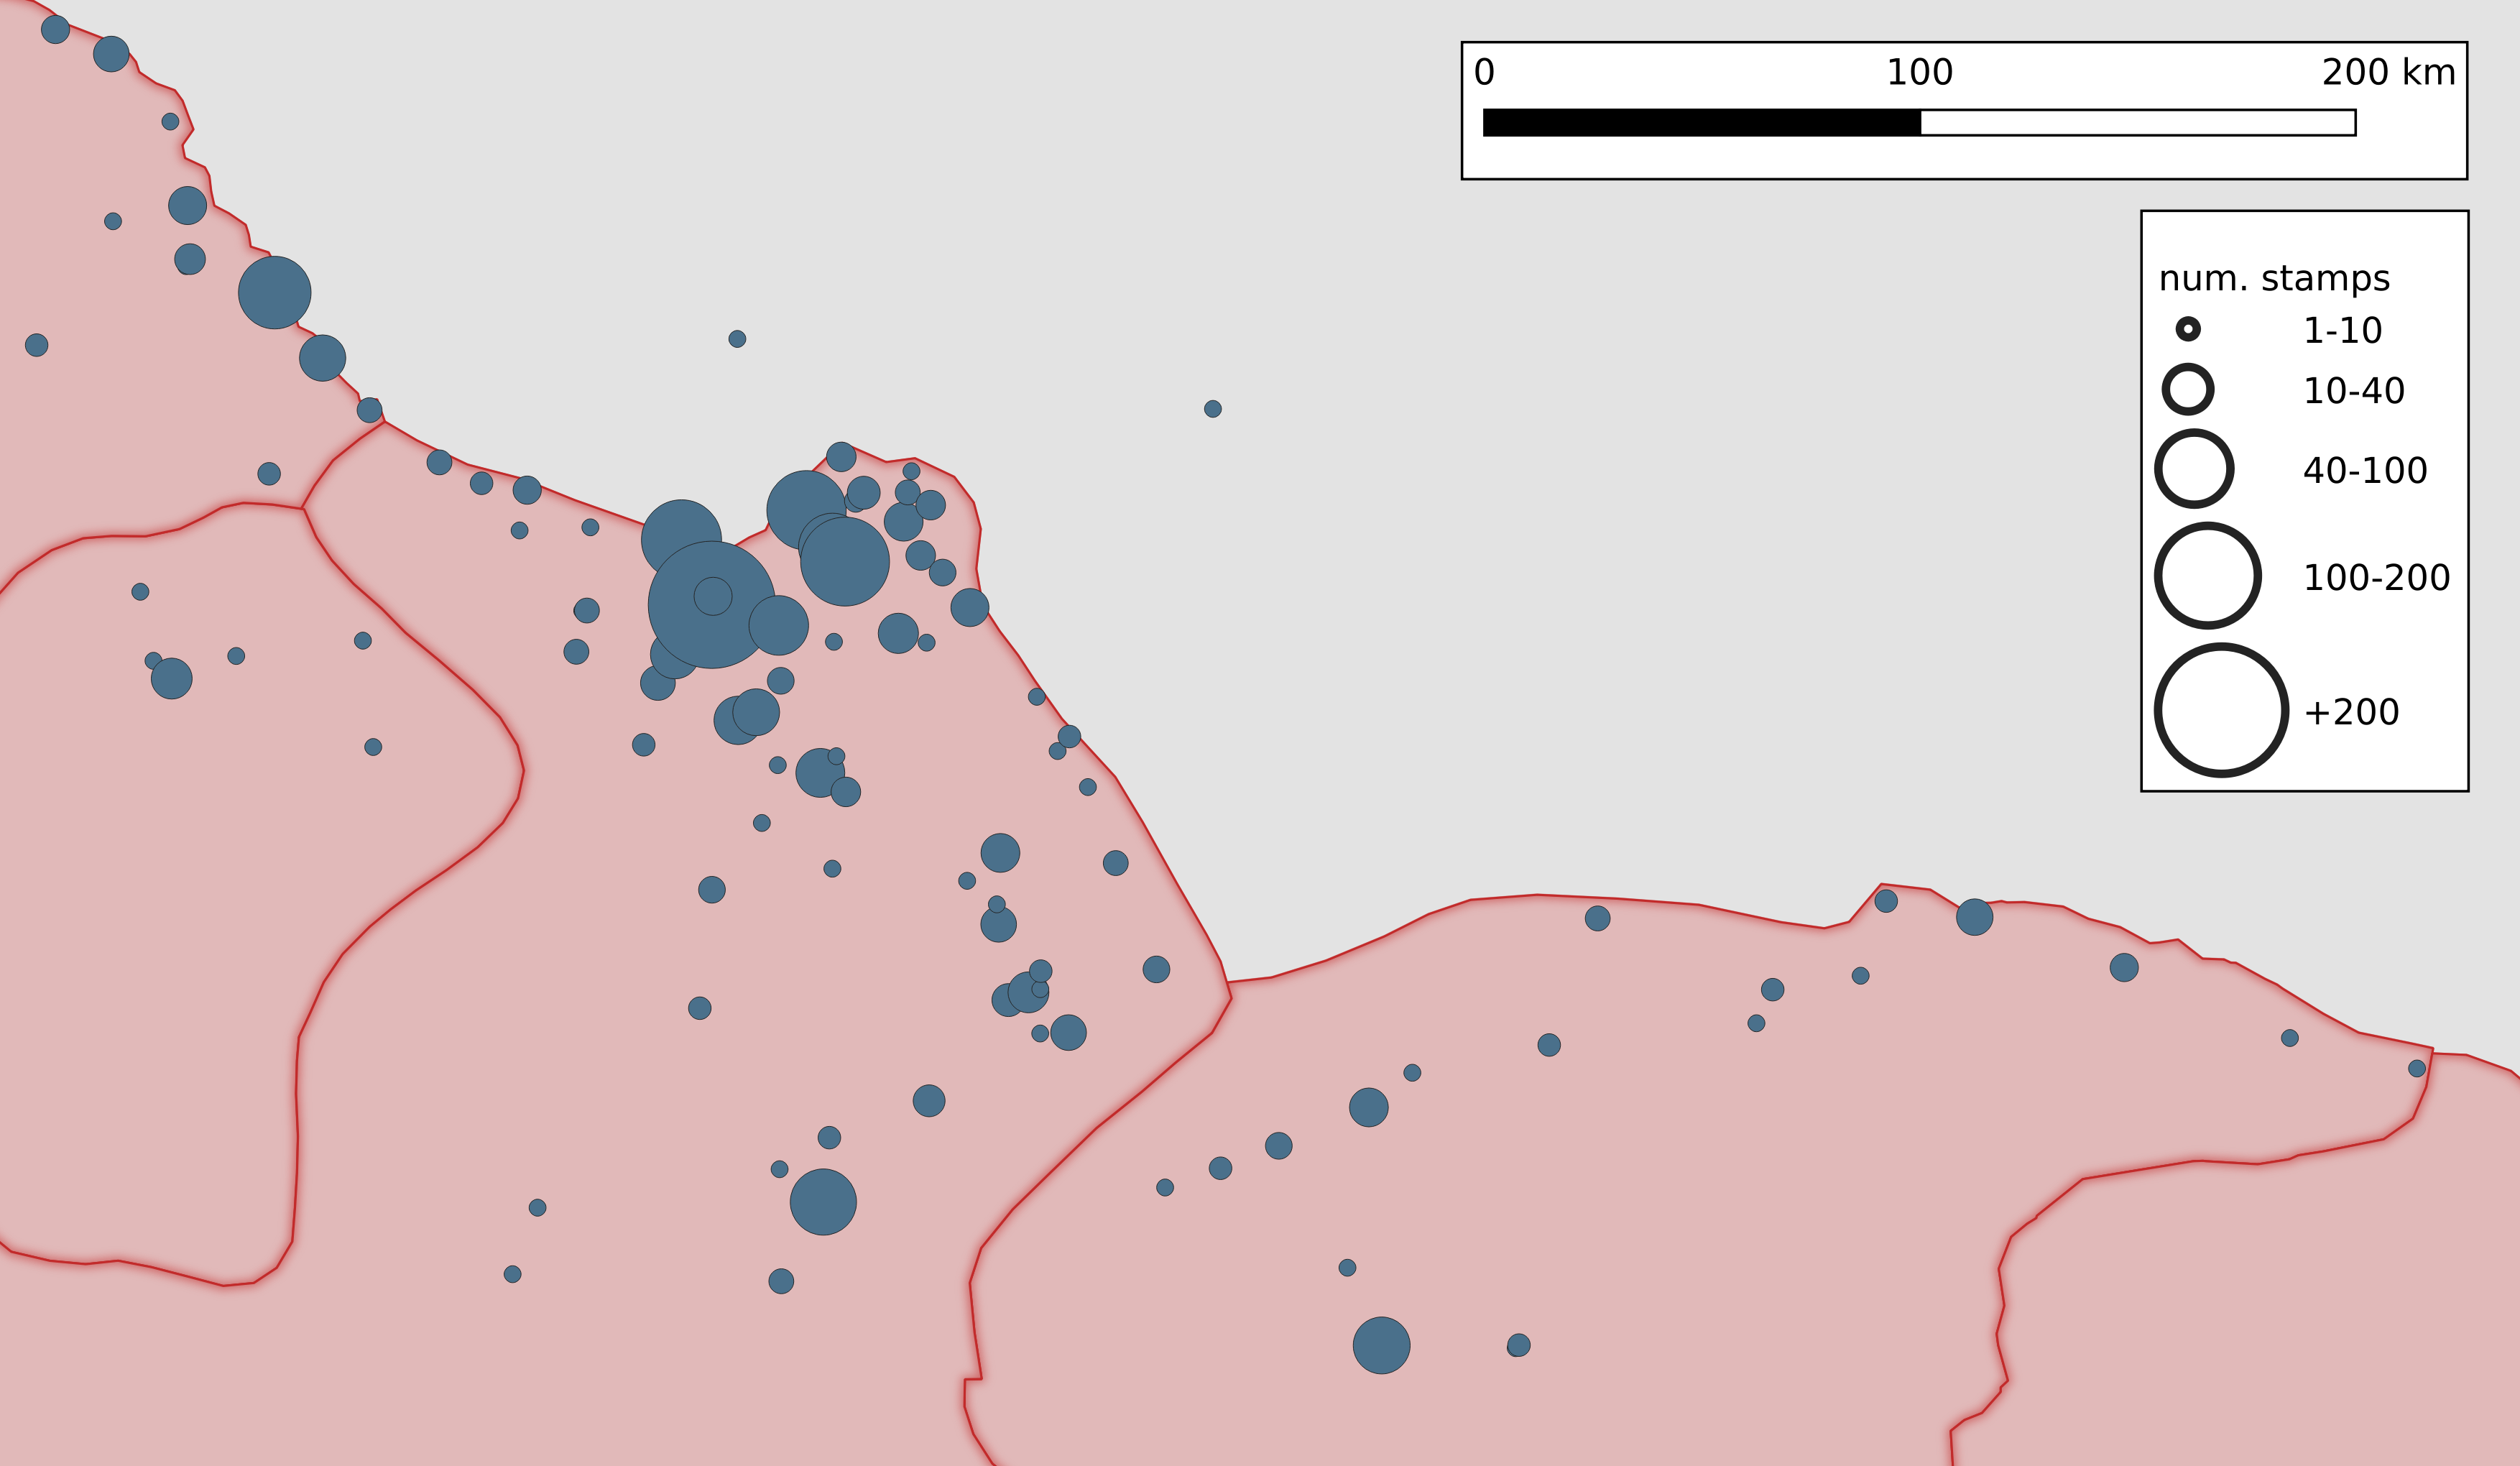
\includegraphics[width=\linewidth]{figs/germania}
\caption{Sites in Germania where Dressel-20 amphoric stamps have been found. Each dot is a site while its size shows the sample size of stamps found in the site. Most sites are located along the German \textit{limes}}
\label{germania}
\end{figure}


\subsection{Measuring the dissimilarity}


%quizás habría que hablar también del filtrado de códigos que se hizo en python porque antes había 3783 stamps pero se filtró por el número de letras...
%\xavi{lo del filtrado lo puedes poner de supplementary information con referencia al antiquity}

The approach proposed here aimed at exploring links between production and consumption centers through the identification of common amphorae codes found in different sites. For this reason we measured the similarity between amphora workshops and/or consumption sites by quantifying a pairwise distance or dissimilarity index between places (i.e. to what extent the stamp codes found on these sites were different). The chosen dissimilarity measure was the Morisita-Horn index \citep{morisita_measuring_1959, horn_measurement_1966}. This method was applied to measure the dissimilarity between different samples of sets. Generally, it describes the dissimilarity between the system of two communities based on the idea of inverse correlation between diversity and species \citep{magurran_why_1988}\xavi{citar reforzar más esta idea}.

The formula can be described as follows \citep{magurran_measuring_2013}:

\begin{equation}
D(MH) = 1- \frac{2 \sum(a_{i} \cdot b_{i})}{(d_{a} + d_{b}) \cdot (N_{a} \cdot N_{b})}
\end{equation} \\

$d_{a}$ and $d_{b}$ are given by the following equation:

\begin{equation}
d_{a} = \frac{\sum a_{i}^{2}}{N_{a}^{2}} 
\end{equation} \\

where $N_{a}$ is the total number of stamps in workshop A; $N_{b}$ is the total number of stamps in workshop B; $a_{i}$ is the number of different stamps for workshop A and $b_{i}$ is the number of different stamps for workshop B.

Considering our dataset as a non-uniform sample, this method provides a useful tool to handle large samples with different sizes and diversity \citep{wolda_similarity_1981}. Morisita-Horn index gives a value between 0 (sites have an exact stamp codes and frequency distribution) and 1 (complete difference between stamp codes). To apply Morisita-Horn we firstly calculated the number of times that each stamp code appeared in an amphora workshop. This method allowed us to bear in mind a similar number of times for each repeated stamp per workshop\xavi{no entiendo esta frase}. If two workshops hhad similar stamp code distribution then the distance index would be close to 0 whereas sites with completely unrelated stamp codes would give a distance close to 1.

\subsection{Hierarchical clustering}

The Morisita-Horn index was used to generate a dissimilarity matrix containing the distance value between each pairwise site based on their code stamps. Hierarchical clustering was applied to this matrix in order to group sites with similar stamps codes distributions. The algorithm was selected to cluster similar groups in order to analyse the relationship between groups of sites and the distribution of similar stamp codes. The results were visualised using a dendrogram to detect groups of sites sharing similar stamp codes.  

\xavi{hasta aquí}

\section{Results}

\subsection{Production centres: Baetica Province}

%The correlation coefficients range from a minimum to a maximum.

The analysis shows that the similarity of amphoric stamps could be correlated with spatial distance. The dendrogram in Fig. \ref{dendro} was obtained with Morisita-Horn index. The dendrogram suggests that amphora workshops used different stamps for their production system. Nearby workshops show similarity on the stamps while most workshops seem to display different stamps. Groups of workshops sharing similar stamps were not found in the dendrogram: the majority of stamp grouping was composed of no more than three workshops. Additionally, workshops that shared more similar amphoric stamps belonged to the same \textit{conventus} area, such as Picachos, Cerro de los Pesebres and El Castillejo. 

\begin{sidewaysfigure}[htp]
	\centering
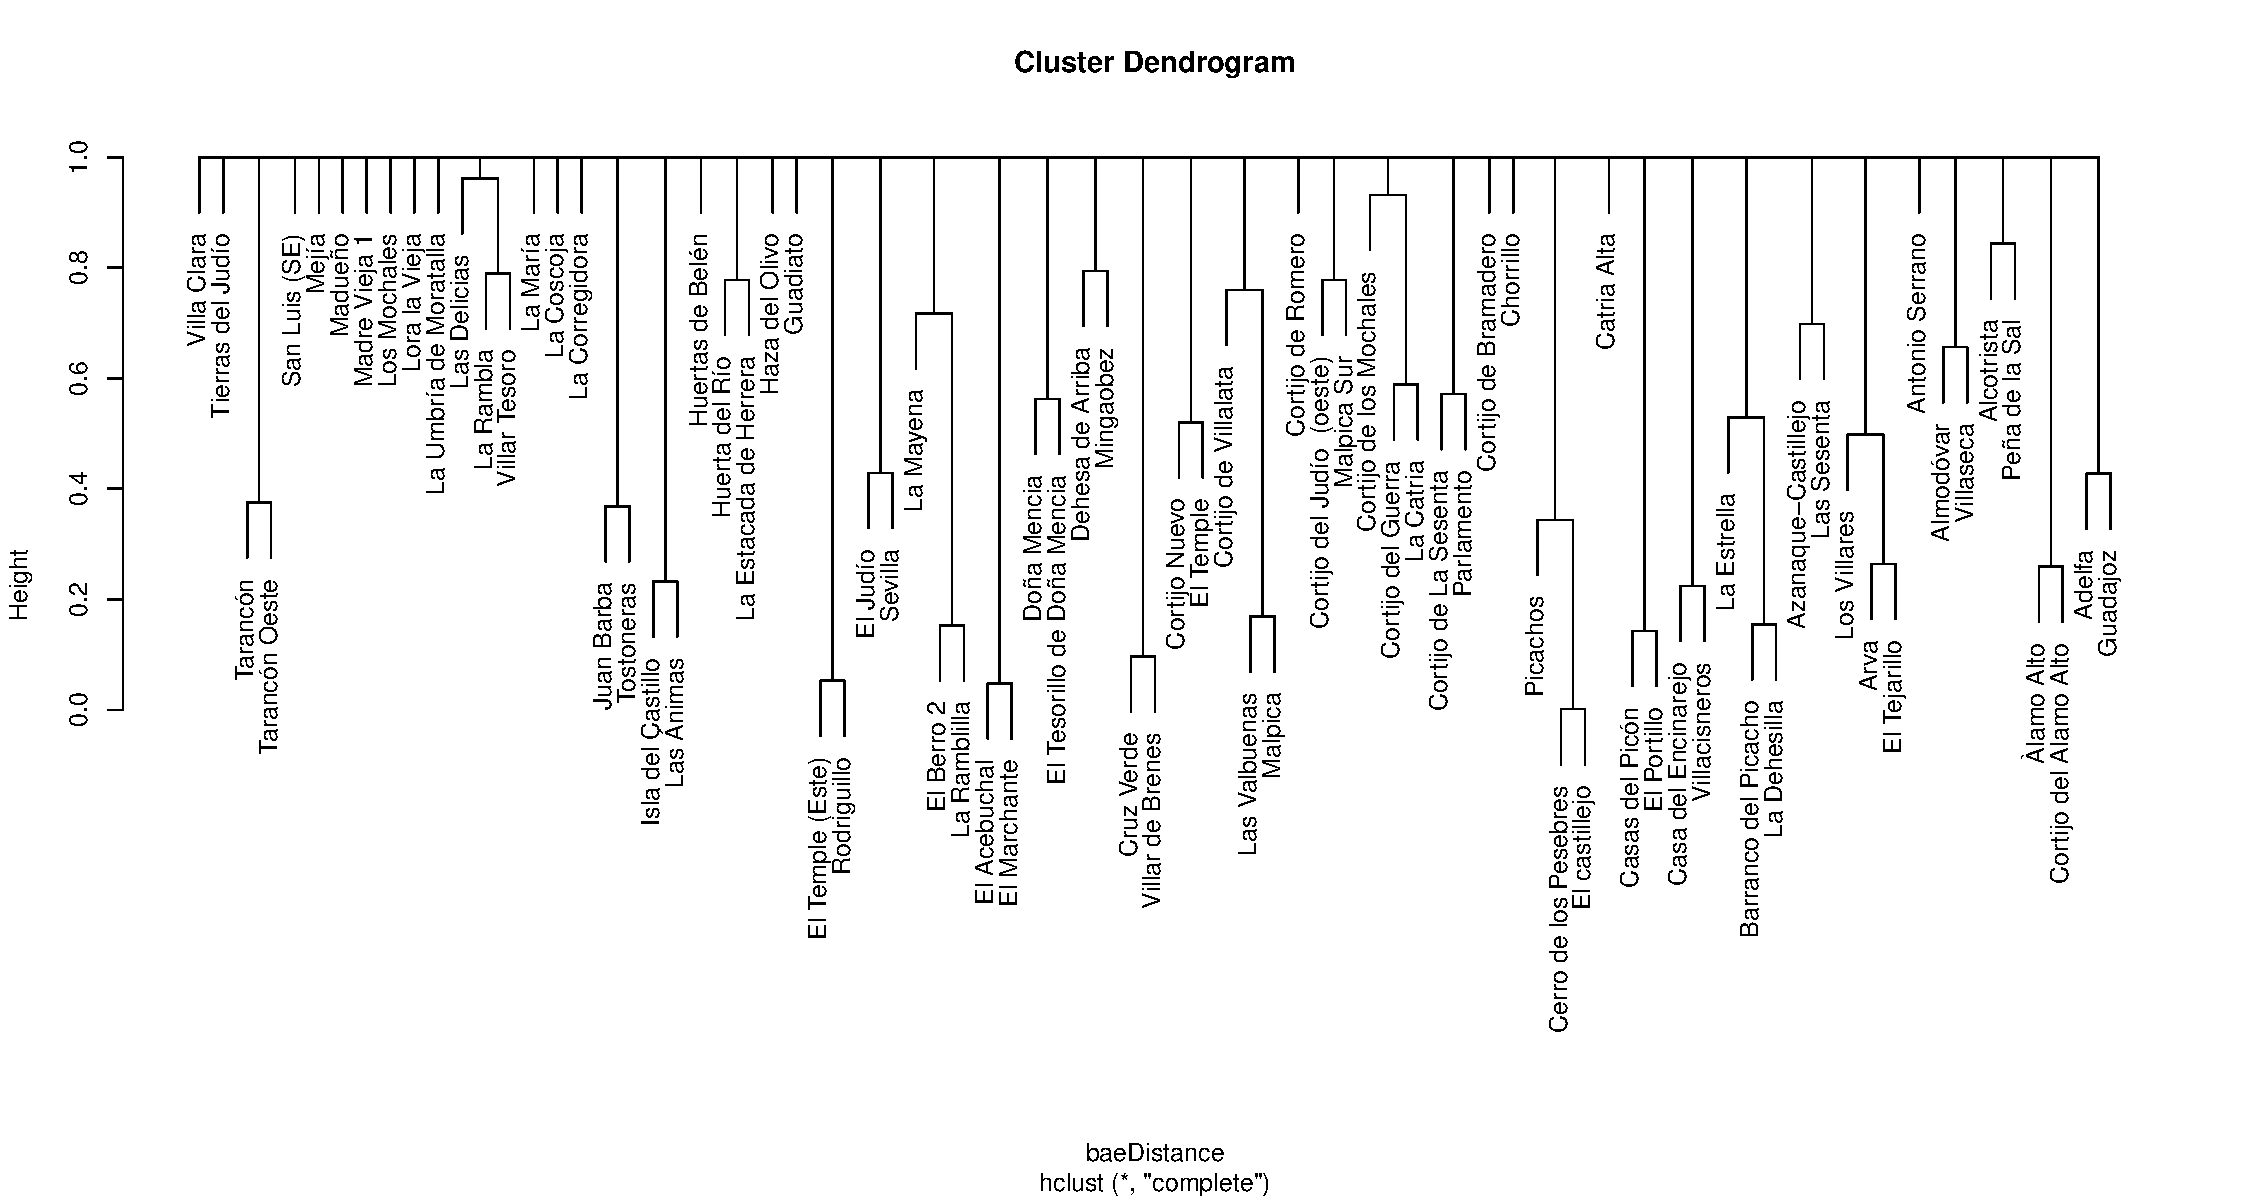
\includegraphics[angle=180, width=\linewidth]{figs/dendro}
\caption{Dendrogram obtained by Morisita-Horn algorithm of different amphora workshops in \textit{Baetica} area. Colours are represented by areas divided into \textit{Hispalis} (red), \textit{Astigi} (green) and \textit{Corduba} (blue)}
\label{dendro}
\end{sidewaysfigure} 


\subsection{Consumption centres: Britannia and Germania}


The results show a similarity with the results obtained in \textit{Baetica} province. However, the similarity is less pronounced as we observed in the dendrogram in Fig. \ref{britmap}

%\xavi{no tengo claro que le puedas decir correlación, porque eso es un valor específico entre 2 distribuciones numéricas. Te refieres a similaridad?}

\begin{sidewaysfigure}[htp]
	\centering
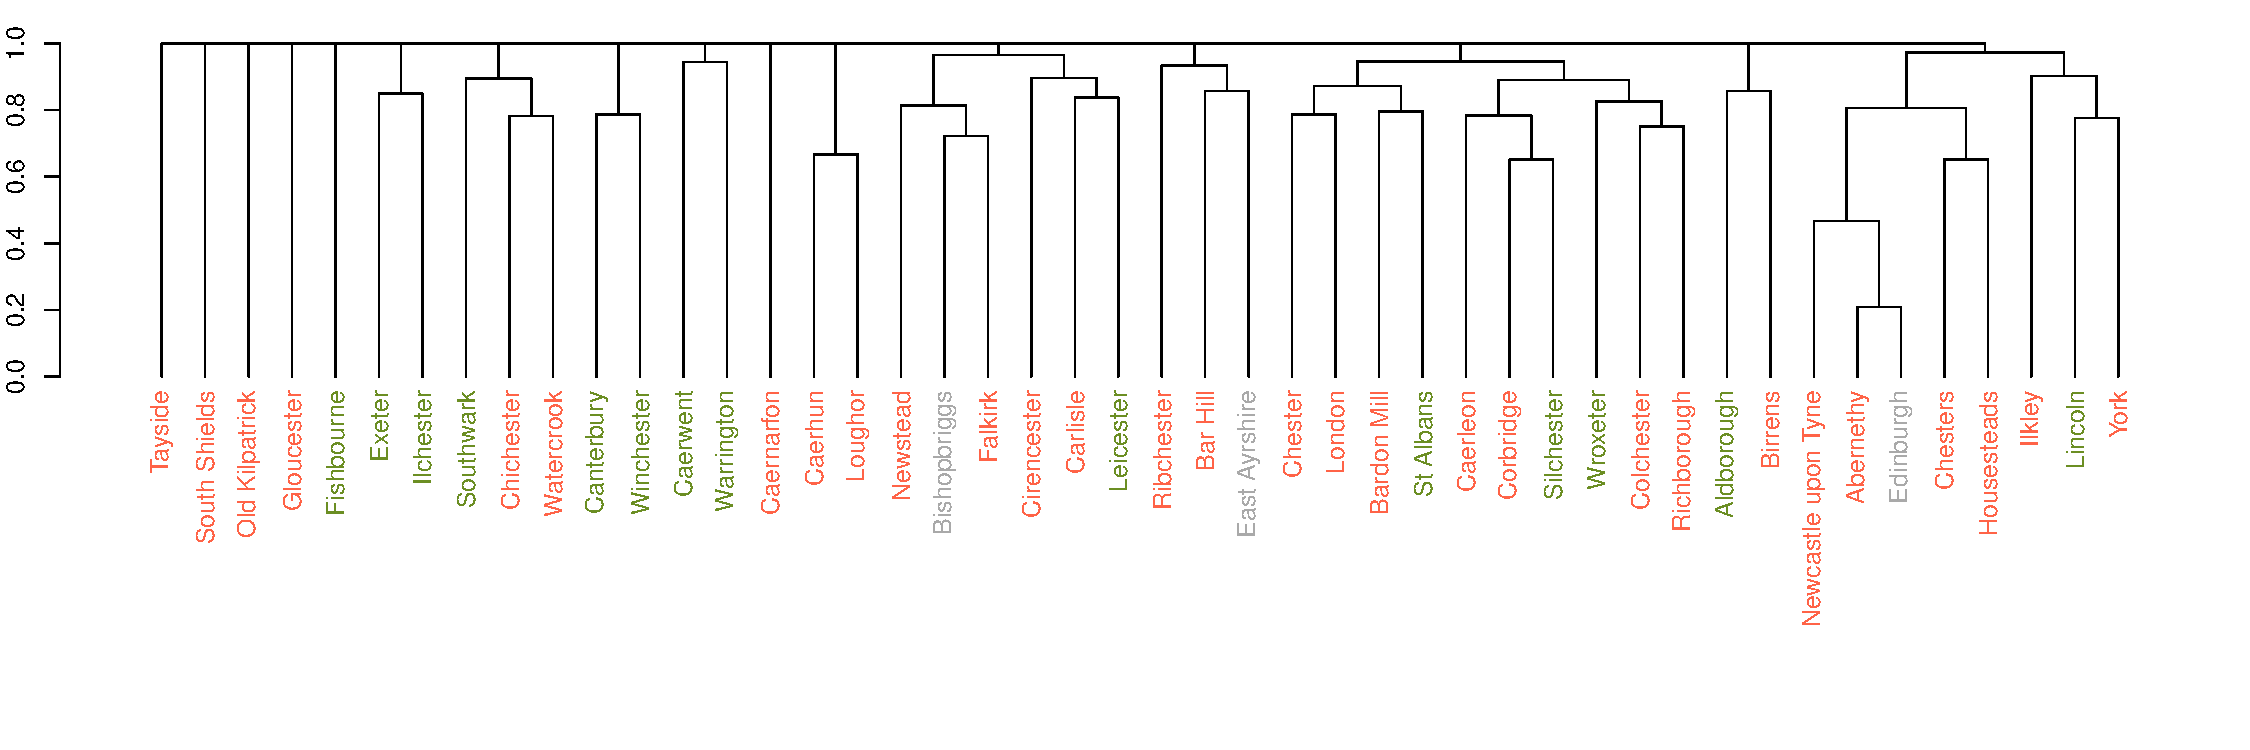
\includegraphics[angle=180,width=\linewidth]{figs/dendrobrit5.pdf}
\caption{Dendrogram obtained by Morisita-Horn algorithm of different sites in \textit{Britannia}. Colours are represented by type of sites divided into military sites (red), civil sites (green) and no specific (grey)}
\label{britmap}
\end{sidewaysfigure}


A minor correlation can be explained by the fact that \textit{Britannia} spatial area is much wider than \textit{Baetica} where the centres were more concentrated.

Most military sites that showed a high similarity in the results were geographically close. We identified two factors: 1) nearby sites tend to share similar stamps and 2) most sites have different stamps. 
By contrast, most sites did not show a strong similarity in stamp correlation. Neither we found a grouping of similar stamps in a specific place. In general, the dendrogram did not observe any production pattern that indicates a clear organisation between production centres and consumption centres. In other words, our results did not indicate the presence of a specific production centre from \textit{Baetica} in \textit{Britannia} province. Rather, it would imply that olive oil production was distributed by non-specific production centres. 


In \textit{Germania}, the similarity of stamps shows results less significant than \textit{Britannia} province as it can be seen in the dendrogram (Fig. \ref{germap}). 

\begin{sidewaysfigure}[htp]
	\centering
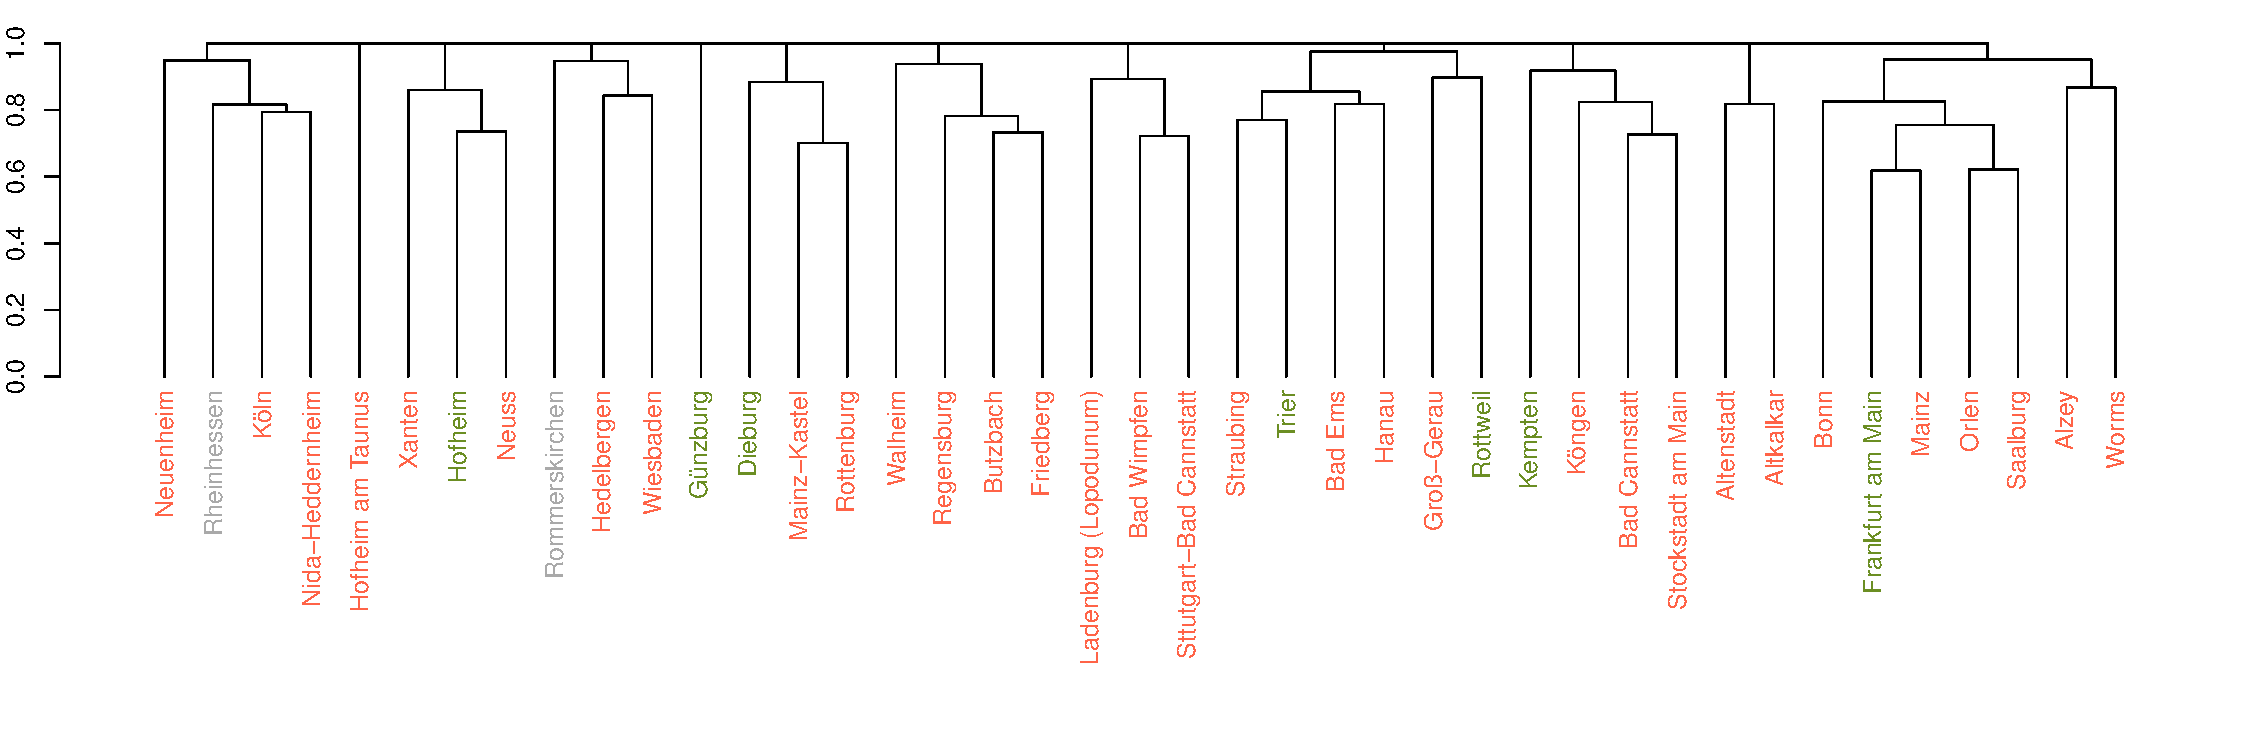
\includegraphics[angle=180, width=\linewidth]{figs/dendroger5.pdf}
\caption{Dendrogram obtained by Morisita-Horn algorithm of different sites in \textit{Germania}. Colours are represented by types of sites divided into military sites (red), civil sites (green) and no specific (grey)}
\label{germap}
\end{sidewaysfigure}

A higher concentration of sites sharing similar stamps were found in areas eminently militarised and close to German \textit{limes}, even if most sites mostly showed different stamps.
The interpretation of the results suggests that there is still no possibility to determine the existence of a defined pattern that reflects in more detail the route of this production in the area of the German limes.


\section{Discussion}


In this work, we aimed to analyse the distribution of the amphoric stamps in the organisation of the olive oil market both in the production and consumption areas. For this reason, an index of dissimilarity was used to detect differences between the distribution of the amphoric stamps and the spatial distance of producers and consumption centres. The general purpose was to explore if such differences found in the stamp codes could play an important role in the Roman market.  

\subsection{Production centres}

The analysis of the amphora workshops in \textit{Baetica} province resulted in a significant correlation between spatial distance and the similarity of the amphoric stamps. 

The analysis suggests a connection between the same stamp code and nearby amphora workshops, excluding certain exceptions. Consequently, the majority of stamps are located in different amphora workshops and only similar stamps between closer amphora workshops were found. Indeed, our results show that most similar stamps were detected in the same \textit{conventus} area. This results may indicate a grouping of stamps with similar codes in the same \textit{conventus}. Despite these stamps tend to share the same area of production, we do not identify groups of any more than three workshops sharing the same amphoric stamps as the dendrogram showed. In general, the majority of stamps were located in different amphora workshops. 

Our results indicate that the hypothesis about groups of amphora workshops sharing the same stamps seems do not match with the results of the analysis, even though there are similar stamps in closer workshops. Rather, it seems that each workshop was organised independently with different stamps. Those stamps detected in closer workshops do not move from other distant workshops. In other words, the stamps tend to remain in the same area and different stamps were located in a same amphora workshop. 

This could be defined by several factors. First, each workshop had a different organisation involved in the use of stamps and they were not used in other workshops. Second, stamp similarity in closer workshops could be linked to a spatial pattern. It is more probably than closer workshops tend to share more traits than distant workshops. While the role of the river was significant for the distribution of amphorae, river connection amongst workshops does not seem to show relevancy for the distribution of stamps. Finally, the distribution of stamps could have shown some research bias. In some cases, workshops have been catalogued with different names in spite of belonging to the same workshops or being closer between each other. Additionally, most of the workshops were not widely excavated. 


\subsection{Consumption centres}

Both consumption centres showed a correlation between spatial distance and similarity in the amphoric stamps. In the case of\textit{Britannia}, the correlation was higher than \textit{Germania}.

In \textit{Britannia}, the majority of similarity stamps were mainly found in military centres. This could be also interpreted by a intense bias where military centres have been mostly excavated than civil centres. 

It should be noted that centres with a similarity correlation were located close to the Atlantic coast around the North Sea and the Celtic Sea. This may indicate that the Atlantic route could have played an essential role in transporting olive oil to the area of \textit{Britannia}, since in the places where there is greater similarity they are found in different strategic points near the sea.

This fact seems to concur with the latest research that suggests the idea of a more important Atlantic route that would connect the militarised provinces \citep{remesal_annona_1986,
remesal_provincial_2008,
carreras_atlantic_2012,
morillo_hispania_2016,rubio-campillo_provincias_2018}.

Therefore, most part of the centres where similar stamps are shared can correspond to eminently military areas, which may mean that the transport could reach the military areas from the beginning and then be distributed by land routes along with other civil areas \citep{carreras_britannia_1998,
ayllon_olive_2018}.

In \textit{Germania}, the results followed the same pattern as \textit{Britannia} but with a minor correlation as we can observe in the dendrogram. The areas mostly militarised share similar stamps than civil areas. However, we do not detect a concrete pattern regarding the distribution of the stamps in the German limes \citep{xanten2018}. 

It is worth to mention that it was not detected a robust model of organisation in both cases with regard to the distribution of stamps in consumption centres. This evidence means that it is unknown whether some production centres went to one province or another or, at least, that they can be clearly reflected in the data with a greater similarity in the amphoric stamps. Thus, production centres could have distributed randomly olive oil both \textit{Britannia} and \textit{Germania}. Neither we do not detect production centres dedicated to the distribution of olive oil in a certain province. 

%In general, we observed a concentration of the stamps in military centres. 

Judging by the results obtained, there does not seem to be a specific pattern in terms of geographical distribution. Nor it was detected consumption areas where stamps are specified from an amphora workshop. 


\section{Concluding remarks}


The results of this work can be interpreted for several reasons. On the one hand, the use of amphoric stamps could have been exclusively running by the owner or owners of the workshop to distinguish the amphora workshop. This hypothesis would explain the fact that we do not find similar stamps in different workshops; however, different code stamps have been detected in the same workshops that they would be barely difficult to assign to different owners.

On the other hand, the presence of different stamps in the same workshop could imply some kind of organisation from within the workshop affecting the closest centres \citep{juanmorostesis}. The marked amphorae could have allowed to potters organise the production with a batch stamping for the posterior commercialisation.  

This could be explained such as batch systematic organisation between potters \citep{juanmorostesis}. 
This method allowed to potters organises the production with the batch stamping for the posterior commercialisation.

Considering that Dressel 20 was not marked in most cases, some researchers point out that potters marked the amphorae to prepare and distribute the product in order to be shipped \citep{berni_millet_epigrafianforica_2008}. This method would be used as an identifier to count the number of amphorae of a branch \citep{juanmorostesis}. This organisation could also have served to identify different groups of potters working in the same amphora workshop. Potters could have marked the amphorae to distinguish different groups working in parallel \citep{li_crossbows_2014}. This fact would explain wherefore why we detect different stamps in the same workshop. In any case, we do not have enough archaeological evidence that can validate the interpretations presented here and our results are only certainly valid with the context of our case study. 

As a summary, this method presented here provides a potential tool to understand the mechanisms of production based on the similarity of artefacts. This work has identified differences in the case of the amphoric production within the Roman Empire. The combination of archaeological data and quantitative methods have finally highlighted for the interpretation of the complex economic processes connected with the archaeological evidence. 


\section{Acknowledgements}

The research was funded by European Research Council Advanced Grant EPNet (340828). We are grateful to Simon Carrignon, Juan Moros and Ignacio Morer for their useful suggestions.  
All data has been analysed and conducted in R program version 3.2.4, using the packages \textit{vegan} \citep{oksanen_vegan_2007}, \textit{ggplot2} \citep{ggplot2:_2016}. Source and code are available at \maria{incluir github}. 


\section{References}

%\bibliography{bibliotex}
\bibliography{bibtesis}



\end{document}
